%!TEX root = origin.TEX
\chapter{Materiales y Métodos}
\pagenumbering{arabic}
\setcounter{page}{11}
\renewcommand{\baselinestretch}{1.2} %doble espacio paratodo el texto

\section{Marco Teórico} 

En este capítulo se presenta una reseña del material bibliográfico investigado con relación a los temas considerados en esta investigación. Los conocimientos investigados son muy amplios, principalmente aquel que ayudó a consolidar las bases del conocimiento científico para elaborar esta tesis, como lo son los temas de aprendizaje artificial profundo, redes neuronales convolucionales, metaheurísticas, procesamiento de imágenes, conocimientos sin los cuales sería difícil de modelar y solucionar computacionalmente cualquier tipo de problema de reconocimiento de imágenes.

\subsection{Antecedentes de la Investigación}

	En este capítulo se presentan 8 trabajos previos con relación a al tema abordado en la investigación y que sirven de base para este.
	\vskip 0.4cm

	\subsubsection
	{INTERNACIONALES:}
		\citep{VicenBueno2007} en la investigación denominada "Traffic Sign Classification by Image Preprocessing and Neural Networks", propusieron clasificar 9 tipos de señales de tráfico de circulación (color azul) de España utilizando una combinación de diferentes técnicas de pre-procesamiento de imágenes junto con una red perceptron de 2 capas la cual produjo un acierto de 98.72\% sobre un conjunto de 78 imágenes para la evaluación. El orden de aplicación de técnicas de pre-procesamiento de imágenes es lo más destacable de este antecedente, recomendando usar el filtro mediano para suavizar la imagen y ecualización de histogramas.
		\vskip 0.4cm

		\citep{Rocha2010} en su investigación "Sistema de Visión Artificial para la Detección y el Reconocimiento de Señales de Tráfico basado en Redes Neuronales", diseñaron un sistema de detección basado en redes neuronales feedfoward y descriptores de forma conocidos como momentos invariantes. Este sistema fue capaz de entrenarse con algunas señales de tránsito con la meta de asistir al conductor de no cometer una infracción o en el peor de los casos un accidente, reconociendo una señal de tránsito a cierta distancia para que así el conductor a priori tenga el conocimiento de esta. El sistema fue implementado en MATLAB y presentó mejorías frente a sistemas basados en lógica difusa o basados únicamente en procesamiento de imágenes, sin embargo, la tasa de acierto no es tan buena obteniéndose un 88.6\% y se recomendó buscar otro método de invarianza que conjuntamente a una red neuronal pueda conseguir mejores resultados. Así el antecedente contribuye a descartar algunos métodos que no puedan presentar mejoras en el reconocimiento de señales de tránsito.
		\vskip 0.4cm

		\citep{Krizhevsky2012} en su investigación """The ImageNet Classification with Deep Convolutional Neural Networks", desarrollaron una red neuronal convolucional grande y profunda para clasificar 1,2 millones de imágenes de alta resolución del concurso ImageNet LSVRC-2010 que categorizaban 1000 clases diferentes de imágenes. Como dato destacable utilizaron un método de regularización muy efectivo para evitar el overfitting de la red denominado dropout, que permitió alcanzar mejores tasas de error en la clasificación que las anteriores técnicas en el estado del arte.
		\vskip 0.4cm	

		\citep{Hannan2014} en la investigación realizada en Malasia "Traffic Sign Classification based on Neural Network for Advance Driver Assistance System", elaboraron un sistema con pasos de pre-procesamiento y extracción de características para clasificar señales de tránsito usando una red perceptron multicapa que funcione en diferentes condiciones de luminosidad. Lo destacable de la investigación, aparte de que el sistema fue capaz de superar la mayor parte del efecto de iluminación en las imágenes, es el tiempo computacional requerido para el análisis de una imagen, siendo en promedio 0.134s, sin embargo la tasa de precisión no fue buena obteniéndose un 84.4\% de acierto para un conjunto de evaluación compuesta por 300 imágenes. 
		\vskip 0.4cm	

		\citep{Hai2014} en su artículo "Morphological Classification for Traffic Sign Recognition", propone un nuevo método para el Reconocimiento de Señales de Tránsito usando el Análisis de Componentes Principales (PCA) y una red Perceptron de Multi-Capa (MLP). En este método propuesto, las señales se detectan individualmente a partir de dos componentes, uno es el color y luego se clasifican en tres clases según la forma: círculo, cuadrado y triángulo. Las características basadas en PCA de estas señales se utilizarán como entrada para la MLP durante la fase de entrenamiento o para responder a clases previamente determinadas. Como contribución resaltante, este enfoque no sólo redujo el tiempo, sino que también aumentó el rendimiento en el proceso de reconocimiento. En la simulación, el método propuesto fue evaluado con más de 500 imágenes y su tasa de precisión llegó a cerca del 96\%. 

		\vskip 0.4cm	
		Como antecedente más relevante para clasificación de señales de tránsito es el realizado en base a datos de Alemania, GTSRB (German Traffic Sign Benchmark) cuenta con más de 50 mil imágenes a color distribuidas en 43 clases, dicha base de datos ha sido tomada como base en la realización de estudios de diferentes métodos tales como: Clasificación basada en la Representación Dispersa (Sparse Representation-based Classification), el algoritmo de Vecinos Más Cercanos (Nearest Neightbor Classifier), Máquina de Soporte de Vectores (Support Vector Machine), entre otros. El mejor resultado fue usando redes neuronales convolucionales \citep{Ciresan}.
		Este conjunto de datos refleja las fuertes variaciones en la apariencia visual de las señales debido a la distancia, la iluminación, las condiciones climáticas, las oclusiones parciales y las rotaciones. %Las imágenes se complementan con varios conjuntos de características precalculadas para permitir, de ser necesario, la aplicación de algoritmos de aprendizaje automático sin conocimientos básicos en el procesamiento de imágenes.
		\vskip 0.4cm

		%\citep{Ciresan}, utilizó una arquitectura que consistía en 3 capas convolucionales usando 100, 150 y 250 filtros cuyos tamaños por cada capa fueron de 42x42, 18x18 y 6x6 neuronas respectivamente, 3 capas pooling con estructuras parecidas a la convolucionales y 1 capa totalmente conectada compuesta por 300 neuronas de entrada para las 43 neuronas de salida que representaban a cada clase.
		%\vskip 0.4cm
		\begin{figure}[H]
		\begin{center}
		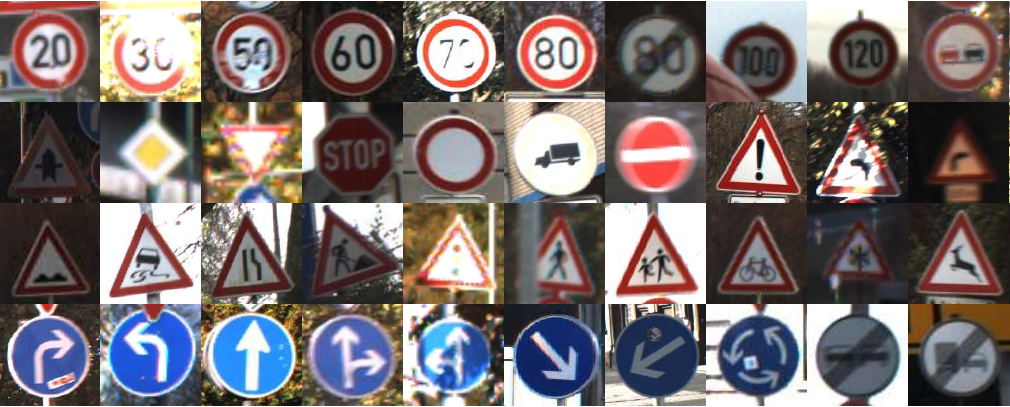
\includegraphics[width=0.7\textwidth]{images/intro/GTSRB}
		\end{center}
		\begin{center}
		\caption{\small{Algunas muestras de la base de datos GTSRB }}
		{\small{Fuente: \cite{Stallkamp2012}}}
		\end{center}
		\vspace{-1.5em}
		\end{figure}

		Los resultados sobre la base de datos GTSRB produjeron un acierto del 99.46\% para el conjunto de imágenes evaluadas, \citep{Stallkamp2012}; sin embargo, desde entonces se han propuesto nuevas variantes de redes neuronales convolucionales, ya sea usando funciones de activación diferentes, usando más capas en la red, mas filtros o introduciendo nuevos métodos de optimización. Lo importante del antecedente es que servirá como elemento de comparación para la investigación propuesta. 


	\newpage		
	\subsubsection
	{NACIONALES:}

		\citep{Vargas2015} en su tesis ”Implementación de un Sistema Inteligente para el Reconocimiento de Señales Preventivas de Seguridad vial", desarrolló un sistema basado enteramente en procesamiento de imágenes para la detección y el reconocimiento de señales de tránsito del tipo preventivas, usando para la detección la técnica de segmentación por color y luego un análisis por la forma y posteriormente para el reconocimiento se usó el algoritmo Speed Up Robust Features (SURF). Todo el proceso fue implementado utilizando la herramienta OpenCV, obteniéndose un acierto del 88\% en un total de 100 señales evaluadas. De este antecedente se analizará la importancia de introducir la segmentación por color al modelo de reconocimiento que se pretende elaborar.
		\vskip 0.4cm

		\citep{Ayuque2016} en su tesis "Diseño de un sistema de clasificación de señales de tránsito vehicular utilizando redes neuronales convolucionales", diseñó 6 modelos de arquitecturas de redes convolucionales para clasificar diversas señales de tránsito de Alemania usando el dataset GTSRB, de los cuales el mejor resultado logró un acierto de 95.29\% en un total de 12630 señales evaluadas, cercano al 99.46\% \citep{Ciresan}. Lo importante del antecedente es que servirá como elemento de comparación para la investigación propuesta. 
		

%***********************************************************************************************************
%***********************************************************************************************************%***********************************************************************************************************

\section{Aprendizaje Profundo} 
	En los primeros días de la inteligencia artificial, el campo atacó y resolvió rápidamente problemas que son intelectualmente difíciles para los seres humanos, pero relativamente sencillos para las computadoras, problemas que pueden describirse mediante una lista de reglas formales y matemáticas. El verdadero desafío para la inteligencia artificial fue y es resolver las tareas que son fáciles de realizar para las personas pero difíciles de describir de manera formal, problemas que resolvemos intuitivamente, que se sienten automáticos, como reconocer palabras, rostros u objetos en las imágenes \citep{Goodfellow-et-al-2016}.

	
	Si bien aprendizaje automático (del inglés, {\bf machine learning}) se describe a menudo como una subdisciplina de la inteligencia artificial(IA), es mejor considerarla como la mejor técnica de la disciplina; es decir, es el campo de la IA que hoy en día muestra la mayor promesa al proporcionar herramientas que la industria y la sociedad pueden usar para producir algún cambio, \citep{Goodfellow-et-al-2016}. En tal sentido, el aprendizaje automático toma algunas de las ideas centrales de la inteligencia artificial y las enfoca en resolver problemas del mundo real con redes neuronales diseñadas para imitar nuestra propia toma de decisiones; sin embargo, el {\bf aprendizaje profundo} o avanzado de máquinas (del inglés, {\bf deep learning}) se centra aún más estrechamente en un subconjunto de herramientas y técnicas del aprendizaje automático y los aplica a la solución de casi cualquier problema que requiera "pensamiento", ya sea humano o artificial \citep{Goodfellow-et-al-2016}.

	
	El aprendizaje profundo es un enfoque específico utilizado para construir y entrenar redes neuronales para la toma de decisiones altamente prometedoras. Se considera que un algoritmo es profundo si los datos de entrada se pasan a través de una serie de no linealidades o transformaciones no lineales antes de que se emita. Este enfoque permitir que las computadoras aprendan de la experiencia y entiendan el mundo en términos de una jerarquía de conceptos, con cada concepto definido a través de su relación con conceptos más simples. Al reunir el conocimiento de la experiencia, este enfoque evita la necesidad de que los operadores humanos especifiquen formalmente todo el conocimiento que necesita la computadora. La jerarquía de conceptos permite que la computadora aprenda conceptos complicados mediante la construcción de los más simples. Si dibujamos un gráfico que muestra cómo estos conceptos se construyen uno encima del otro, el gráfico es profundo, con muchas capas. Por esta razón, este enfoque se conoce como el aprendizaje profundo de la inteligencia artificial \citep{Goodfellow-et-al-2016}.

	
	El aprendizaje profundo elimina el hecho que se tenga que realizar una identificación manual de las características en los datos y, en cambio, depende del proceso de capacitación que tenga para descubrir los patrones útiles en los ejemplos de entrada. Esto hace que el entrenamiento de la red neuronal sea más fácil y más rápido \citep{Goodfellow-et-al-2016}. Las imágenes son un gran ejemplo de cómo funciona esto, ya que contienen muchos elementos diferentes y no es fácil para nosotros comprender cómo una computadora, con su mente o proceso centrado en el cálculo y direccionado en un solo sentido, puede aprender a interpretarlas de la misma manera que nosotros. Pero el aprendizaje profundo se puede aplicar a cualquier forma de datos (señales de máquina, audio, video, voz, palabras escritas) para producir conclusiones que parecen haber sido alcanzadas por simples humanos.

	
	%\newpage
	Por el contrario, la mayoría de los algoritmos modernos de machine learning se consideran "poco profundos", debido a que la entrada solo puede abarcar unos pocos niveles de llamadas en subrutinas. El rendimiento de estos algoritmos simples de aprendizaje automático depende en gran medida de la presentación de los datos que se les proporcionan. Por ejemplo, cuando se usa la regresión logística para recomendar una cesárea, el sistema de IA no examina al paciente directamente. En cambio, el médico le dice al sistema varias piezas de información relevante, como la presencia o ausencia de una cicatriz uterina. Cada pieza de información incluida en la representación del paciente se conoce como una característica. La regresión logística aprende cómo cada una de estas características del paciente se correlaciona con diversos resultados. Sin embargo, no puede influir en cómo se definen las características de todos modos. Si a la regresión logística se le realizara una resonancia magnética del paciente, en lugar del informe formal del médico, no sería capaz de hacer predicciones útiles. Los píxeles individuales en una exploración de la resonancia tienen una correlación insignificante con cualquier complicación que pueda ocurrir durante el parto. Esta dependencia de las representaciones es un fenómeno general que aparece no solo en la vida cotidiana sino también en las ciencias de la computación. En tal sentido, operaciones como buscar una colección de datos puede avanzar exponencialmente más rápido si la colección está estructurada e indexada de forma inteligente. La gente puede realizar fácilmente números aritméticos arábigos, pero encuentra que la aritmética en números romanos consume mucho más tiempo. No es sorprendente que la elección de la representación tenga un enorme efecto en el rendimiento de los algoritmos de aprendizaje automático \citep{Goodfellow-et-al-2016}.

	
	Para muchas tareas, sin embargo, es difícil saber qué características se deben extraer. Por ejemplo, un programa para detectar automóviles en fotografías. Se sabe que los autos tienen ruedas, por lo que sería importante utilizar la presencia de una rueda como característica. Desafortunadamente, es difícil describir exactamente cómo es una rueda en términos de valores de píxel. Una rueda tiene una geometría simple, pero su imagen puede verse complicada por las sombras que caen sobre la rueda, el sonido de las partes metálicas de la rueda, el guardabarros del automóvil o un objeto en el primer plano que oscurece la rueda, y así sucesivamente. 

	
	Una solución a este problema es utilizar el aprendizaje automático para descubrir no solo el mapeo que inicia en la representación hasta el resultado sino también la representación en sí misma. Este enfoque se conoce como aprendizaje representativo (del inglés, {\bf representation learning}). Las representaciones aprendidas a menudo dan como resultado un rendimiento mucho mejor que el que se puede obtener con representaciones diseñadas a mano. También permiten que los sistemas de IA se adapten rápidamente a nuevas tareas, con una intervención humana mínima. Un algoritmo de aprendizaje de representación puede descubrir un conjunto de características para una tarea simple en minutos o para una tarea compleja en horas. El diseño manual de funciones para una tarea compleja requiere una gran cantidad de tiempo humano y esfuerzo; puede llevar décadas para toda una comunidad de investigadores, \citep{Goodfellow-et-al-2016}.
	
	Al diseñar algoritmos para el aprendizaje de características, el objetivo suele ser separar los factores de variación que explican los datos observados. En este contexto, se usa la palabra "factores", simplemente para referirse a fuentes de influencia separadas; los factores generalmente no se combinan por multiplicación. Tales factores a menudo no son cantidades que se observan directamente. En cambio, pueden existir como objetos no observados o fuerzas no observadas en el mundo físico que afectan las cantidades observables. También pueden existir como constructores en la mente humana que proporcionan una simplificación útil de las explicaciones o causas inferidas de los datos observados. Pueden considerarse como conceptos o abstracciones que nos ayudan a dar sentido a la rica variabilidad de los datos. Al analizar una grabación de voz, los factores de variación incluyen la voz del hablante, su sexo, su acento y las palabras que están hablando. Al analizar la imagen de un automóvil, los factores de variación incluyen la posición del automóvil, su color y el ángulo y el brillo del sol.
	
	Una fuente importante de dificultad en muchas aplicaciones de inteligencia artificial del mundo real es que muchos de los factores de variación influyen en cada pieza de datos que podemos observar. Los píxeles individuales en una imagen de un automóvil rojo pueden ser muy cercanos al negro en la noche. La forma de la silueta del automóvil depende del ángulo de visión. La mayoría de las aplicaciones nos exigen separar los factores de variación y descartar las que no nos interesan. Por supuesto, puede ser muy difícil extraer tales características abstractas de alto nivel a partir de datos en bruto. Muchos de estos factores de variación, como el acento de un hablante, solo se identifican mediante una comprensión sofisticada y casi humana de los datos. Cuando es casi tan difícil obtener una representación como para resolver el problema original, el aprendizaje de la representación, a primera vista, no parece ayudarnos.
	
	El aprendizaje profundo resuelve este problema central en el aprendizaje representativo mediante la introducción de representaciones que se expresan en términos de otras representaciones más simples. El aprendizaje profundo permite a la computadora construir conceptos complejos a partir de conceptos más simples. La Figura 2.2 muestra cómo un sistema de aprendizaje profundo puede representar el concepto de una imagen de una persona combinando conceptos más simples, como esquinas y contornos, que a su vez se definen en términos de bordes.
		\begin{figure}[H]
		\begin{center}
		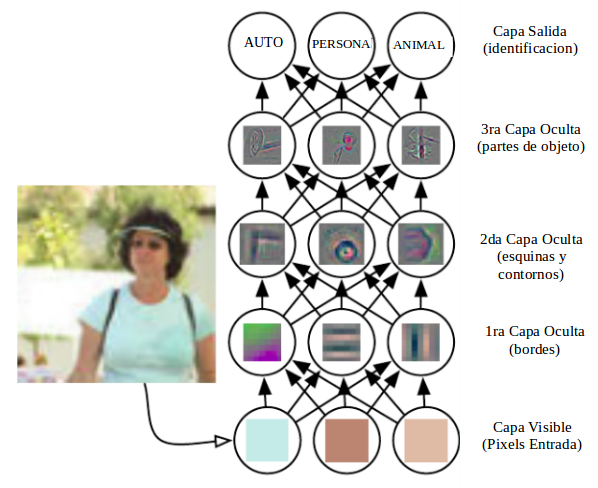
\includegraphics[width=0.7\textwidth]{images/marcoteorico/deepExam}
		\end{center}
		\begin{center}
		\caption{\small{Ilustración de un modelo de aprendizaje profundo}}
		\vskip -0.25cm
		{\small{Fuente: \cite{Goodfellow-et-al-2016}}}
		\end{center}
		\vspace{-1.5em}
		\end{figure}
	\vskip 0.4cm 
	La idea de aprender la representación correcta de los datos proporciona una perspectiva para el aprendizaje profundo, \citep{Goodfellow-et-al-2016}. Otra perspectiva del aprendizaje profundo es que la profundidad permite que la computadora aprenda un programa de computadora de varios pasos. Cada capa de la representación se puede considerar como el estado de la memoria del computador después de ejecutar otro conjunto de instrucciones en paralelo. Las redes con mayor profundidad pueden ejecutar más instrucciones en secuencia. Las instrucciones secuenciales ofrecen gran poder porque las instrucciones posteriores pueden referirse a los resultados de instrucciones anteriores. De acuerdo con esta visión del aprendizaje profundo, no toda la información en las activaciones de una capa necesariamente codifica los factores de variación que explican la entrada. La representación también almacena información del estado que ayuda a ejecutar un programa el cual puede dar sentido a la entrada. Esta información de estado podría ser análoga a un contador o puntero en un programa informático tradicional. No tiene nada que ver con el contenido de la entrada específicamente, pero ayuda al modelo a organizar su procesamiento.
	\vskip 0.4cm 
	Hay dos formas principales de medir la profundidad de un modelo, \citep{Goodfellow-et-al-2016}. La primera vista se basa en la cantidad de instrucciones secuenciales que se deben ejecutar para evaluar el modelo. Podemos considerar esto como la longitud de la ruta más larga a través de un diagrama de flujo que describe cómo calcular cada una de las salidas del modelo a partir de sus entradas. Otro enfoque, utilizado por modelos probabilísticos profundos, considera que la profundidad de un modelo no es la profundidad del gráfico computacional sino la profundidad del gráfico que describe cómo los conceptos se relacionan entre sí. En este caso, la profundidad del diagrama de flujo de los cálculos necesarios para calcular la representación de cada concepto puede ser mucho más profunda que la gráfica de los conceptos mismos. Esto se debe a que la comprensión del sistema de los conceptos más simples puede ser refinado dada la información sobre conceptos más complejos.
	\vskip 0.4cm 
	Debido a que no siempre está claro cuál de estos dos puntos de vista (la profundidad del gráfico computacional o la profundidad del gráfico de modelado probabilístico) es más relevante, y debido a que diferentes personas eligen diferentes conjuntos de elementos más pequeños para construir sus gráficos, no hay un solo valor correcto para la profundidad de un modelo, así como no hay un solo valor correcto para la longitud de un programa de computadora. Tampoco hay consenso sobre la profundidad que requiere un modelo para calificar como "profundo", \citep{Goodfellow-et-al-2016}. Sin embargo, el aprendizaje profundo puede considerarse con seguridad como el estudio de modelos que implican una mayor cantidad de composición de funciones o conceptos aprendidos en comparación con el aprendizaje automático tradicional.
	\vskip 0.4cm 
	En resumen, el aprendizaje profundo, es un enfoque a la IA; específicamente, es un tipo de aprendizaje automático, una técnica que permite que los sistemas computacionales mejoren con la experiencia y los datos. En este sentido, se puede sostener que el aprendizaje automático es el único enfoque viable para construir sistemas de inteligencia artificial que puedan operar en entornos complicados del mundo real y el aprendizaje profundo es un tipo particular de aprendizaje automático que logra gran poder y flexibilidad al representar el mundo como una jerarquía de conceptos anidados, con cada concepto definido en relación a conceptos más simples y representaciones más abstractas calculadas en base a representaciones menos abstractas. La siguiente imagen es un diagrama de Venn que muestra cómo el aprendizaje profundo es una especie de aprendizaje de representación, que a su vez es una especie de aprendizaje automático que se utiliza para muchos de los enfoques de la IA. 

	\begin{figure}[H]
		\begin{center}
		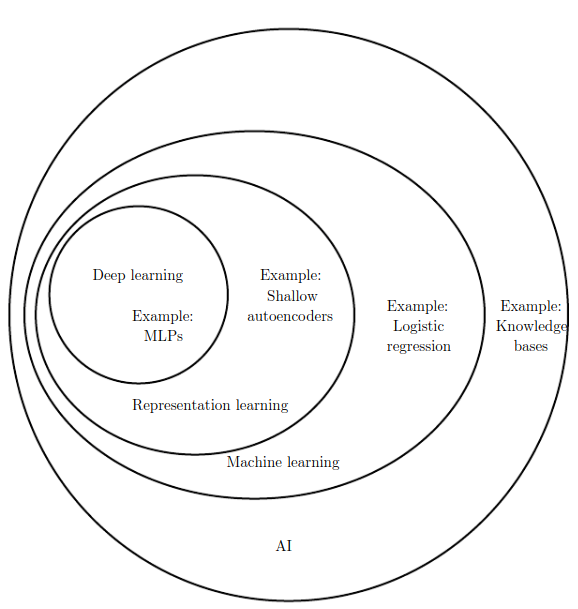
\includegraphics[width=0.8\textwidth, height=12.5cm]{images/marcoteorico/venn_diag}
		\end{center}
		\begin{center}
		\vskip -0.1cm
		\caption{\small{Diagrama de Venn donde cada sección incluye un ejemplo de una tecnología de IA (ilustra la relación entre estas diferentes disciplinas de la IA)}}
		{\small{Fuente: \cite{Goodfellow-et-al-2016}}}
		\end{center}
		\vspace{-1.5em}
		\end{figure}

\section{Red Convolucional} 

	Nueve de cada diez veces, cuando se escucha que el aprendizaje profundo rompe una nueva barrera tecnológica, las redes neuronales convolucionales están involucradas. También llamados CNN (del inglés, {\bf Convolutional Neural Networks}) o  {\bf ConvNets}, estas son las preferidas del campo de redes neuronales profundas. Han aprendido a clasificar las imágenes en categorías incluso mejor que los humanos en algunos casos, \citep{Rohrer}.
	
	\vskip 0.4cm  
	Los modelos de redes convolucionales siempre suponen explícitamente que las entradas deben ser mapeadas en forma de imágenes, lo que nos permite configurar parte inicial de las propiedades o características del modelo a diseñar.  Debido a esta característica la limitación de las ConvNets radica en que solo capturan patrones espaciales locales en datos. Es decir, si no se puede hacer que los datos se vean como una imagen, las ConvNets son prácticamente muy poco útiles, \citep{Rohrer}.

	\vskip 0.4cm  
	Las redes neuronales convolucionales son muy similares a las redes neuronales ordinarias, están formadas por neuronas que tienen pesos y biases (sesgos) que pueden aprender información durante el entrenamiento de estas. Cada neurona recibe algunas entradas y realiza operaciones matemáticas. Toda la red expresa una única función de puntuación diferenciable: desde el contenido de los píxeles de la imagen en un extremo(entrada) hasta los puntajes que definen la clase o resultado correspondiente en el otro extremo(salida).

	\begin{figure}[H]
	\begin{center}
	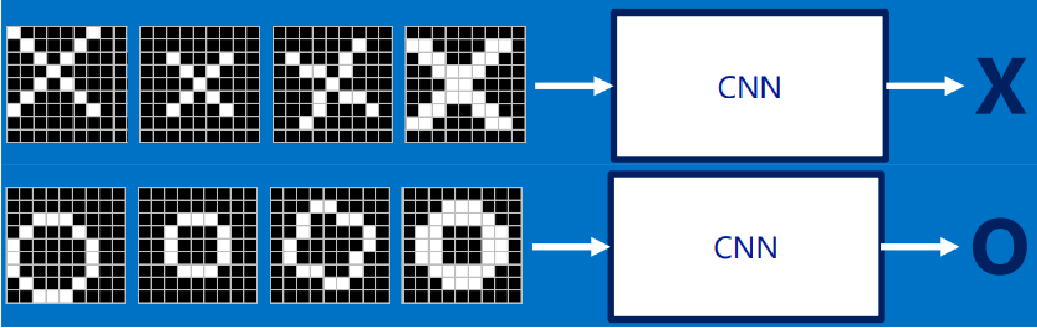
\includegraphics[width=0.7\textwidth]{images/marcoteorico/entr_salida}
	\end{center}
	\begin{center}
	\caption{\small{Entrada y salida de una CNN}}
	\vskip -0.25cm
	{\small{Fuente: \cite{Rohrer}}}
	\end{center}
	\vspace{-1.5em}
	\end{figure}

	El resultado de las CNNs es que pueden encontrar si una característica está en una imagen sin preocuparse exactamente de donde está. Esto ayuda a resolver el problema de las computadoras al comparar imágenes de manera híper-literal, es decir, que coincida pixel a pixel para que se trate de imágenes iguales.

	\begin{figure}[H]
	\begin{center}
	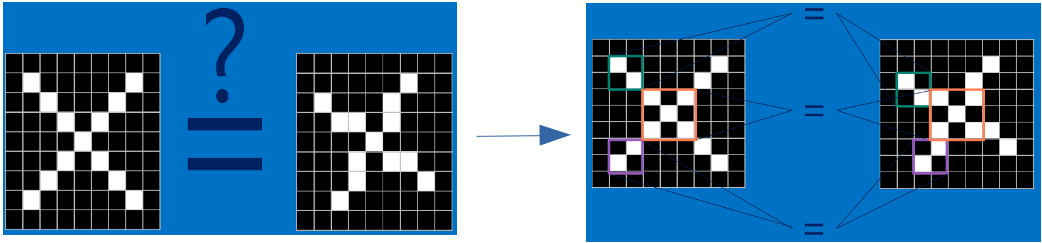
\includegraphics[width=0.8\textwidth]{images/marcoteorico/literalcomp}
	\end{center}
	\begin{center}
	\caption{\small{Análisis de una CNN}}
	\vskip -0.25cm
	{\small{Fuente: \cite{Rohrer}}}
	\end{center}
	\vspace{-1.5em}
	\end{figure}

	Una ConvNet se caracteriza por tener una secuencia de capas donde cada una de estas transforma un volumen de activaciones en otro nuevo a través de funciones y el aprendizaje profundo se produce cuando se utilizan varias de estas capas variando los parámetros de configuración dentro y entre dichas capas. 
	\vskip 0.4cm  
	Existen dos conjuntos de terminologías para describir estas capas. Una es cuando la red convolucional es vista como un número largo de capas simples y cada paso del procesamiento se considera como una capa en sí misma. Otra terminología es cuando la red convolucional es vista como un número pequeño de capas relativamente complejas, donde cada capa tiene múltiples etapas. En esta terminología, existe un mapeo directo entre los volúmenes de activaciones y las capas de red. En esta investigación se usará esta terminología.

	
	\begin{figure}[H]
	\begin{center}
	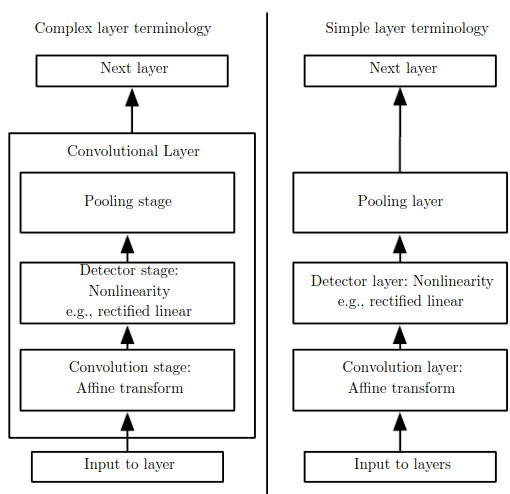
\includegraphics[width=0.6\textwidth]{images/marcoteorico/types}
	\end{center}
	\begin{center}
	\caption{\small{Terminología de capas complejas(izquierda) y de capas simples(derecha)}}
	{\small{Fuente: \cite{Goodfellow-et-al-2016}}}
	\end{center}
	\vspace{-1.5em}
	\end{figure}
	
	\subsection{Capa Convolucional}

		Los parámetros de la capa convolucional consisten básicamente en dos datos. La entrada y todo lo que respecta a un conjunto de filtros (también denominados kernels) cuyos valores se aprenden, es decir, empiezan con datos aleatorios y conforme avance el entrenamiento se van alterando. 
		\vskip 0.3cm 
		\subsubsection {Etapa de Convolución} 
		  
		Para el proceso convolucional cada filtro es pequeño espacialmente (a lo ancho y alto), incluso se extiende a través de la profundidad total del volumen de entrada(imagen). Por ejemplo, un filtro típico en una primera capa de una ConvNet podría tener un tamaño de 5x5x3 (es decir, 5 píxeles de ancho y alto, y 3 de profundidad debido a que los canales de color - RGB). Durante el proceso hacia adelante, se desliza (más precisamente, convoluciona) cada filtro a través del ancho y alto (incluso profundidad) del volumen de entrada para calcular los productos de puntos entre las entradas del filtro y la entrada en cualquier posición.

		\begin{figure}[H]
		\begin{center}
		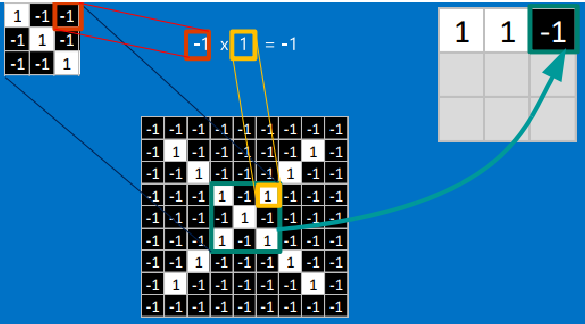
\includegraphics[width=0.75\textwidth]{images/marcoteorico/generate_filt1}
		\end{center}
		\begin{center}
		\caption{\small{Convolución entre el filtro y parte de la imagen}}
		\vskip -0.25cm
		{\small{Fuente: \cite{Rohrer}}}
		\end{center}
		\vspace{-1.9em}
		\end{figure}

		\begin{figure}[H]
		\begin{center}
		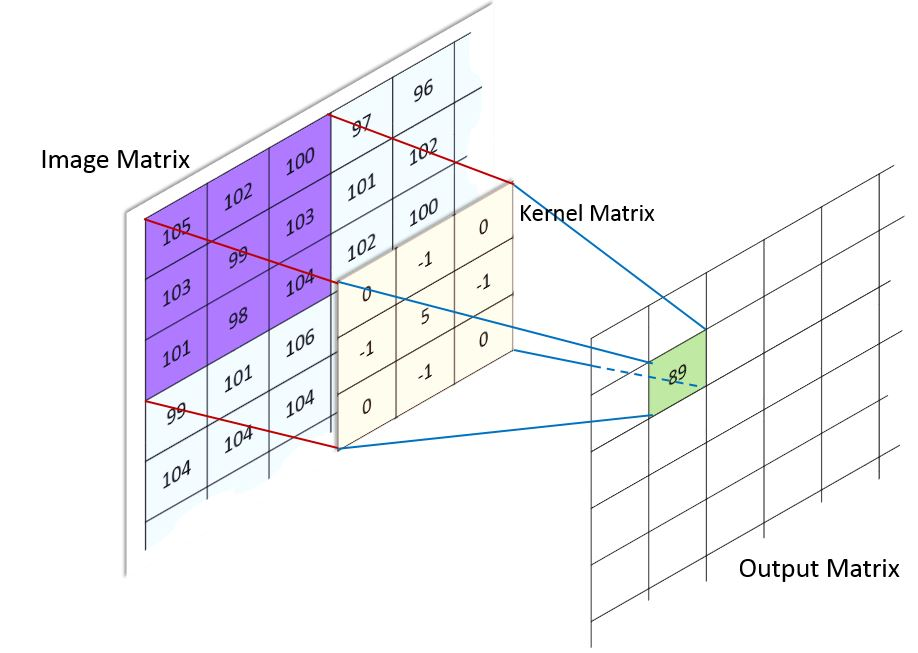
\includegraphics[width=0.75\textwidth]{images/marcoteorico/Convolution_calculation1}
		\end{center}
		\begin{center}
		\caption{\small{Posicionamiento del kernel/filtro por pixel}}
		{\small{Fuente: Elaboración propia}}
		\end{center}
		\vspace{-1.9em}
		\end{figure}

		A medida que deslizamos el filtro sobre el ancho y la altura del volumen de entrada produciremos un mapa de activación bidimensional que proporciona las respuestas de ese filtro en cada posición espacial. Es decir, el proceso en esta capa consiste en calcular la coincidencia de un filtro con una parte de la imagen, y para conseguirlo simplemente se multiplica cada píxel en el filtro por el valor del píxel en la imagen. Para luego, sumar las respuestas y dividirlas por el número total de píxeles en el filtro.

		\begin{figure}[H]
		\begin{center}
		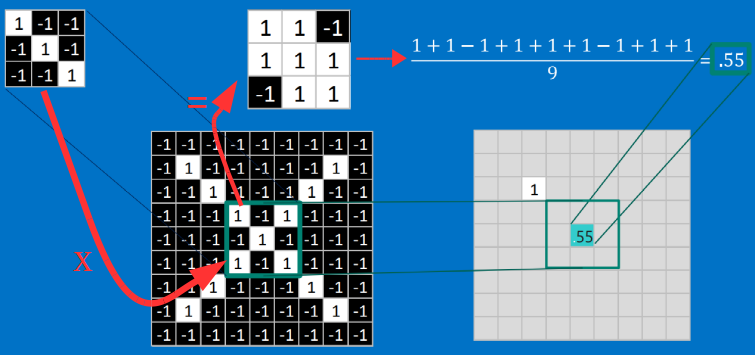
\includegraphics[width=0.75\textwidth]{images/marcoteorico/conv_filt1}
		\end{center}
		\begin{center}
		\caption{\small{Proceso matemático convolucional}}
		{\small{Fuente: \cite{Rohrer}}}
		\end{center}
		\vspace{-1em}
		\end{figure}

		\begin{figure}[H]
		\begin{center}
		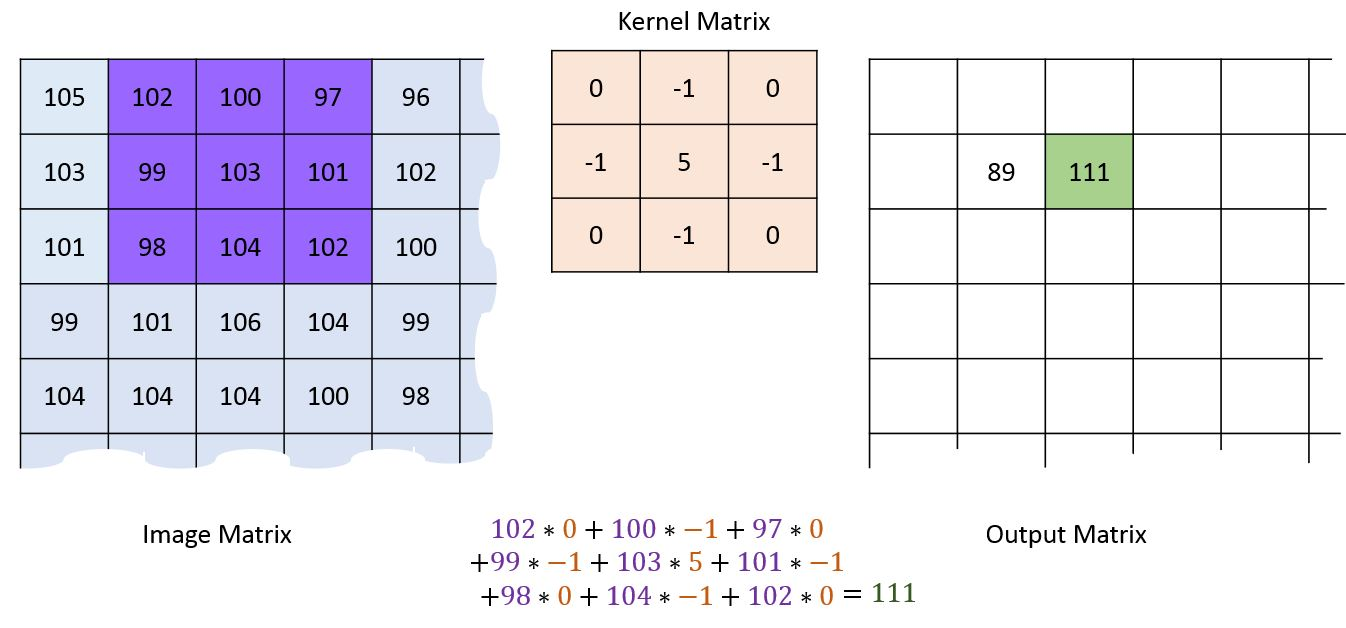
\includegraphics[width=0.75\textwidth]{images/marcoteorico/Convolution_calculation2}
		\end{center}
		\begin{center}
		\caption{\small{Cálculo Convolucional}}
		{\small{Fuente: Elaboración propia}}
		\end{center}
		\vspace{-1.9em}
		\end{figure}

		Cada filtro puede ser representado como una neurona de salida, cuyo valor se halla usando la sumatoria de pesos como se muestra en la figura 2.10. Intuitivamente, la red aprenderá los filtros que se activan cuando ven algún tipo de característica visual, como un borde o contorno en alguna orientación específica. 
		
		\vskip 0.4cm  
		
		La convolución aprovecha tres ideas importantes que pueden ayudar a mejorar un sistema de aprendizaje automático: {\bf interacciones dispersas}, {\bf uso compartido de parámetros} y {\bf representaciones equivalentes}.
		
		\vskip 0.4cm  
		Las capas de redes neuronales tradicionales usan la multiplicación de matrices mediante una matriz de parámetros con un parámetro separado que describe la interacción entre cada unidad de entrada y cada unidad de salida. Esto significa que cada unidad de salida interactúa con cada unidad de entrada. Sin embargo, las redes convolucionales suelen tener {\bf interacciones dispersas} (también conocidas como conectividad dispersa o ponderaciones dispersas), en las cuales el kernel es más pequeño que la entrada. Por ejemplo, al procesar una imagen, la imagen de entrada puede tener miles o millones de píxeles, pero podemos detectar características pequeñas y significativas, como bordes con núcleos que ocupan solo decenas o cientos de píxeles, necesitando almacenar menos parámetros, lo que reduce los requisitos de memoria del modelo, mejora su eficiencia estadística y también conlleva a que el cálculo de la salida requiera menos operaciones.
		\vskip 0.4cm
		Estas mejoras en la eficiencia suelen ser bastante grandes. Si hay entradas({\textit n}) y salidas({\textit m}), la multiplicación de la matriz requiere $n \times m$ parámetros, y los algoritmos utilizados en la práctica por ejemplo tienen complejidad de tiempo de ejecución $O(n \times m)$. Si limitamos el número de conexiones que cada salida puede tener a {\textit k}, entonces el enfoque dispersamente conectado requiere solo $k \times m$ parámetros y $O(k \times m)$ en tiempo de ejecución. Para muchas aplicaciones prácticas, es posible obtener un buen rendimiento en la tarea de aprendizaje automático mientras se mantienen {\textit k} distintos órdenes de magnitud menores que {\textit m}. Para demostraciones gráficas de conectividad dispersa, vea la figura 2.11, donde se resalta una unidad de entrada $x_{3}$, y las unidades de salida que son afectadas por esta unidad. (Arriba) Cuando {\bf {\textit {s}}} está formado por convolución con un kernel de ancho 3, solo tres salidas se ven afectadas por {\bf \textit  x}. (Abajo) Cuando {\bf \textit s} está formado por la multiplicación de la matriz, la conectividad ya no es dispersa, por lo que todos los resultados se ven afectados por $x_{3}$.

		\begin{figure}[H]
		\begin{center}
		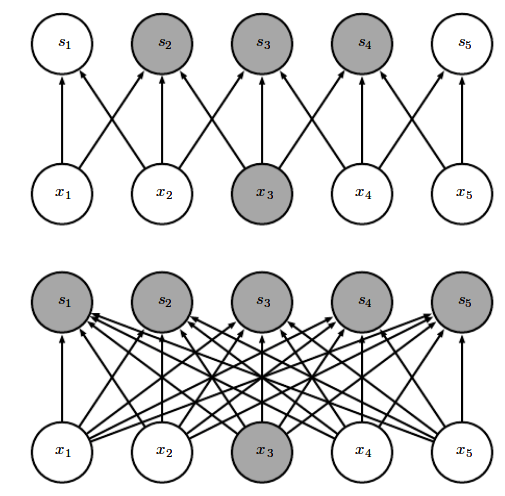
\includegraphics[width=0.5\textwidth]{images/marcoteorico/sparceCon}
		\end{center}
		\begin{center}
		\caption{\footnotesize \small{Conectividad dispersa vs No Dispersa}}
		\vskip -0.2cm  
		{\small{Fuente: \cite{Goodfellow-et-al-2016}}}
		\end{center}
		\vspace{-1.9em}
		\end{figure} 	

		  
		En una red convolucional profunda, las unidades en las capas más profundas pueden interactuar indirectamente con una porción más grande de la entrada. Esto permite que la red describa de manera eficiente las interacciones complicadas entre muchas variables mediante la construcción de tales interacciones a partir de bloques de construcción simples que describen cada una de ellas. Por lo tanto, aunque las conexiones directas en una red convolucional son muy dispersas, las unidades en las capas más profundas pueden conectarse indirectamente a la totalidad o a la mayoría de la imagen de entrada, \citep{Goodfellow-et-al-2016}.
		\begin{figure}[H]
		\begin{center}
		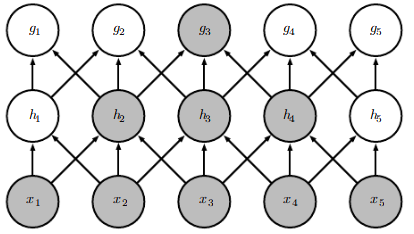
\includegraphics[width=0.5\textwidth]{images/marcoteorico/sparceCondeep}
		\end{center}
		\begin{center}
		\caption{\footnotesize \small{Capacidad receptiva en capas más profundas en una red convolucional}}
		\vskip -0.2cm  
		{\small{Fuente: \cite{Goodfellow-et-al-2016}}}
		\end{center}
		\vspace{-1.9em}
		\end{figure} 	

		
		El uso {\bf compartido de parámetros} hace referencia al uso del mismo parámetro para más de una función en un modelo. En una red neuronal tradicional, cada elemento de la matriz de pesos se usa exactamente una vez cuando se calcula la salida de una capa. Se multiplica por un elemento de la entrada y luego nunca se vuelve a visitar. Como sinónimo de compartición de parámetros, se puede decir que una red tiene ponderaciones vinculadas, porque el valor de la ponderación aplicada a una entrada está vinculado al valor de una ponderación aplicada a otra parte. En una red neuronal convolucional, cada miembro del kernel se utiliza en cada posición de la entrada (excepto tal vez algunos de los píxeles de los bordes, dependiendo de las decisiones de diseño con respecto al límite). El uso compartido de parámetros utilizado por la operación de convolución significa que, en lugar de aprender conjuntos de parámetros para cada ubicación por separado, aprendemos un solo conjunto, \citep{Goodfellow-et-al-2016}.
		\vskip 0.4cm  

		En el caso de la convolución, la forma particular de compartir los parámetros hace que la capa tenga una propiedad llamada {\bf representaciones equivalentes}. Decir que una función es equivalente significa que, si la entrada cambia, la salida cambia de la misma manera.
		La convolución crea un mapa en 2-D de donde aparecen ciertas características en la entrada. Si movemos el objeto en la entrada, su representación se moverá la misma cantidad en la salida. Esto es útil cuando sabemos que se utiliza alguna función de un número pequeño de píxeles vecinos cuando se aplica a ubicaciones de entrada múltiples. Por ejemplo, al procesar imágenes, es útil detectar bordes en la primera capa de una red convolucional. Los mismos bordes aparecen más o menos en todas partes en la imagen, por lo que es práctico compartir los parámetros en toda la imagen.

		\begin{figure}[H]
		\begin{center}
		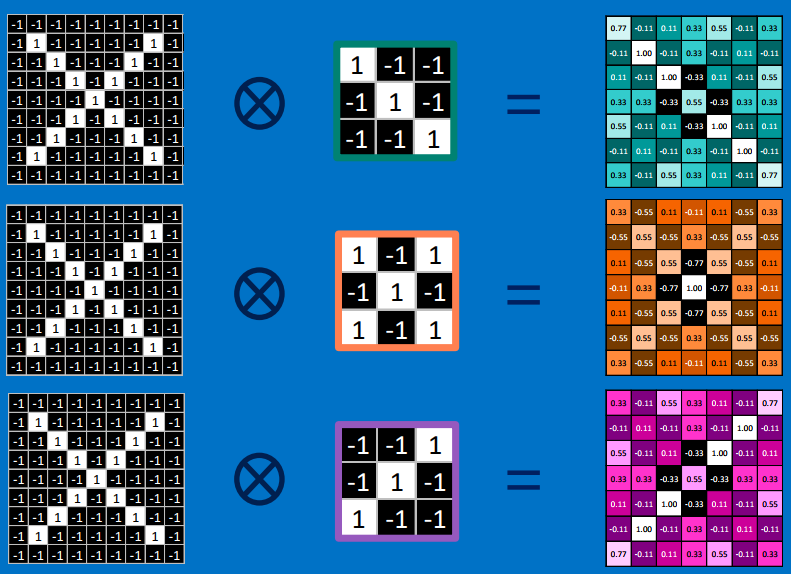
\includegraphics[width=0.6\textwidth]{images/marcoteorico/result_conv}
		\end{center}
		\begin{center}
		\vskip 0.1cm  
		\caption{\small{Resultado de Convolución (conjunto de mapas de activación. generado a partir de 3 filtros para 3 características: diagonal derecha, cruzamiento central y diagonal izquierda). Símbolo de convolución: $\otimes$}}
		\vskip -0.1cm  
		{\small{Fuente: \cite{Rohrer}}}
		\end{center}
		\vspace{-1.9em}
		\end{figure}

		En resumen, se tiene un conjunto completo de 'n' filtros en cada capa convolucional (determinando la profundidad de la capa) y cada uno de estos filtros producirá un mapa de activación bidimensional por separado. Apilaremos estos mapas de activación a lo largo de la dimensión de profundidad y produciremos el volumen de salida, es decir el resultado es un conjunto de imágenes que muestran una versión filtrada de la imagen original resaltando características o patrones importantes de ella, como puede ser visto en la figura 2.13.

		\vskip 0.4cm  
		Cabe resaltar que para la construcción de un filtro o kernel, es necesario considerar tres aspectos importantes: la extensión espacial (spatial extent), el paso (stride) y la cantidad de zero a rellenar (zero-padding).
		\newpage
		
		\begin{enumerate}
			\item La extensión espacial es el tamaño del filtro, comúnmente es de tamaño impar tanto en largo y ancho.
			
			\item El stride es otra pieza del bloque de construcción básico de los filtros convolucionales. Este representa el {\textit 'paso'} en la operación de convolución indicando cuánto es que se debe desplazar un filtro en una imagen con cada paso. El filtro se desliza sobre la imagen, se detiene en cada longitud de salto y realiza las operaciones necesarias en ese paso.

				\begin{figure}[H]
				\begin{center}
				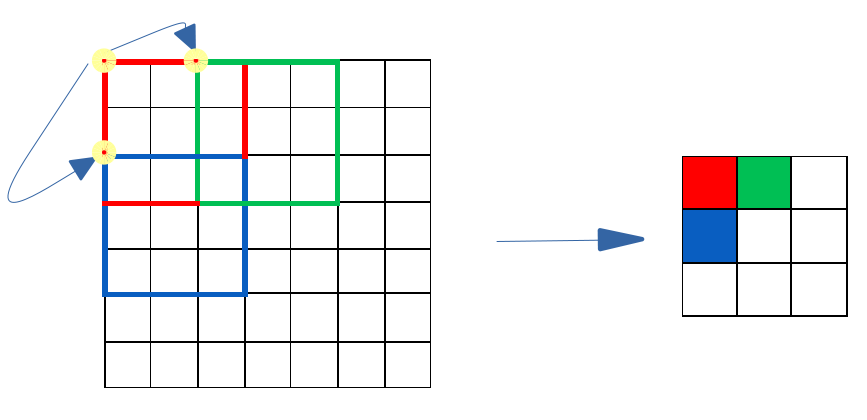
\includegraphics[width=0.55\textwidth]{images/marcoteorico/stride}
				\end{center}
				\begin{center}
				\caption{\small{Imagen con stride igual a 2, para el filtro tanto en largura como anchura}}
				\vspace{-0.5em}
				{\small{Fuente: Elaboración propia}}
				\end{center}
				\vspace{-1.9em}
				\end{figure}
			\item Zero-padding agrega ceros alrededor del borde de una imagen.
				\begin{figure}[H]
				\begin{center}
				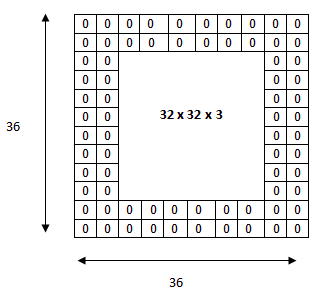
\includegraphics[width=0.4\textwidth]{images/marcoteorico/PAD2}
				\end{center}
				\begin{center}
				\caption{\small{Ejemplo de zero-padding con tamaño 2}}
				\vspace{-0.5em}
				{\small{Fuente: Elaboración propia}}
				\end{center}
				\vspace{-1.9em}
				\end{figure}

				Los principales beneficios del relleno son los siguientes:
				\begin{itemize}
				\item Le permite usar una capa de convolución sin necesariamente reducir la altura y el ancho de los volúmenes. Esto es importante para construir redes más profundas, ya que de lo contrario la altura / ancho se reduciría a medida que se avanza hacia capas más profundas.
				\item Nos ayuda a mantener más información en el borde de una imagen. Sin relleno, muy pocos valores en la siguiente capa se verían afectados por los píxeles como los bordes de una imagen.
				\end{itemize}
			
		\end{enumerate}
		%\vskip 0.4cm  

		\noindent Cada capa convolucional recibe como dato de entrada los parámetros:
		${W_{0}}\times{H_{0}}\times{D_{0}}$ \newline
		Produce un dato de salida con los siguientes parámetros: ${W_{1}}\times{H_{1}}\times{D_{1}}$\newline
		Estas salidas, son influenciadas por la manera de configuración de los filtros.\newline
		\vspace{-2em} 
		
		\begin{minipage}[t]{0.5\textwidth}
		En el que:
		\begingroup\makeatletter\def\f@size{12.4}\check@mathfonts
		\begin{center}
		 ${W_{1}} = \frac{{W_{0}} - F + 2P}{S} +1$ 
		\vskip 0.4cm 
		 ${H_{1}} = \frac{{H_{0}} - F + 2P}{S} +1$ 
		\vskip 0.4cm 
		 ${D_{1}} = K$ 
		 \end{center}
		\endgroup
		\end{minipage}
		%second column
		\begin{minipage}[t]{0.55\textwidth}
		Donde:
		\vskip 0.1cm 
		$W$ es el ancho (width) de la imagen, \vskip 0.4cm  
		$H$ es la altura (height) de la imagen,\vskip 0.4cm 
		$D$ es la profundidad (depth)de la imagen,\vskip 0.4cm 
		$F$ es la extensión espacial (spatial extent) del filtro,\vskip 0.4cm 
		$S$ es el paso (stride) del filtro,\vskip 0.4cm 
		$P$ es la cantidad de zero padding del filtro,\vskip 0.4cm 
		$K$ es el número de filtros (filters).\vskip 0.4cm 
		\end{minipage}
		\vskip 0.4cm 
		\noindent La ecuación de convolución de manera generalizada es:
		
		\begingroup\makeatletter\def\f@size{14.4}\check@mathfonts
		\begin{center}
		${conv_j^n} ={\sum_{k=1}^k x_k^n \times w_{kj} ^n + b_n}$
		\end{center}
		\endgroup
		
		En el que:\vskip 0.1cm
		\begin{itemize}
			\item $x,w,b$ son valores de entrada, pesos y biases (sesgos), respectivamente.
			\item $n$ es el número de la capa
			\item $j$ es el número del filtro de salida
			\item $k$ es la cantidad de filtros en la capa $n-1$ o $n$
		\end{itemize}


		\begin{figure}[H]
		\begin{center}
		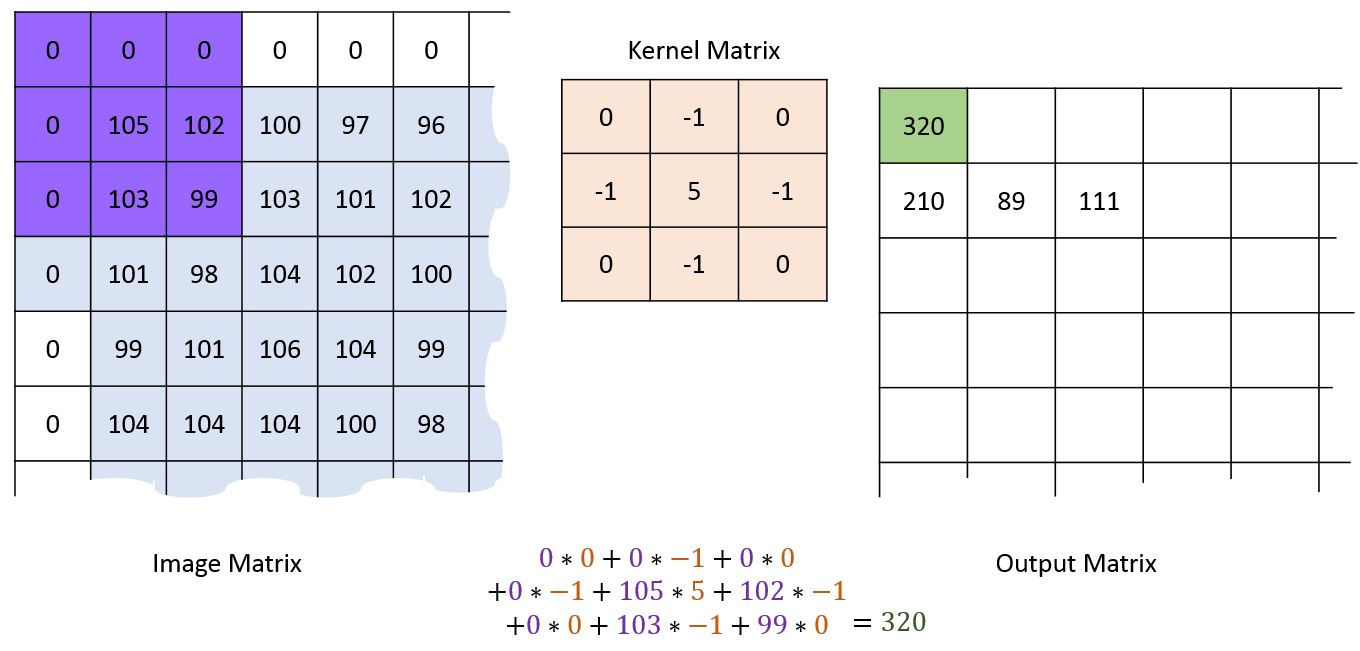
\includegraphics[width=0.75\textwidth]{images/marcoteorico/Convolution_calculation_borders}
		\end{center}
		\begin{center}
		\caption{\small{Ejemplo de filtro creado a partir de los 3 aspectos mencionados}}
		{\small{Fuente: Elaboración propia}}
		\end{center}
		\vspace{-1.9em}
		\end{figure}

		\vskip 0.3cm  
	\subsubsection  {Capa ReLU (Rectified Linear Units)}
		\vskip -0.2cm 
		Debido al hecho que todas las capas en una red neuronal no son lineales, después de calcular los valores para cada una de las neuronas en la red neuronal, colocamos estos valores a través de una función de activación. Una red neuronal artificial consiste básicamente en multiplicaciones y suma de matrices. Si solo utilizáramos estos cálculos lineales, podríamos apilarlos uno encima del otro y esa no sería una red muy profunda. Por lo tanto, a menudo se utiliza funciones de activación no lineales en cada capa de la red. Apilando capas de funciones lineales y no lineales una encima de la otra, teóricamente podemos modelar cualquier problema.
		\vskip 0.2cm 
		Estas son las tres funciones de activación no lineal más populares:
		\begin{enumerate}
		\item[1)] Sigmoid (analiza un valor entre 0 y 1)  \vspace{-0.5em}
		\item[2)] TanH (analiza un valor entre -1 y 1) \vspace{-0.5em}
		\item[3)] ReLU (si el valor es negativo, se convierte en 0, de lo contrario, permanece igual) \vspace{-0.5em}
		\end{enumerate}

		\begin{figure}[H]
		\begin{center}
		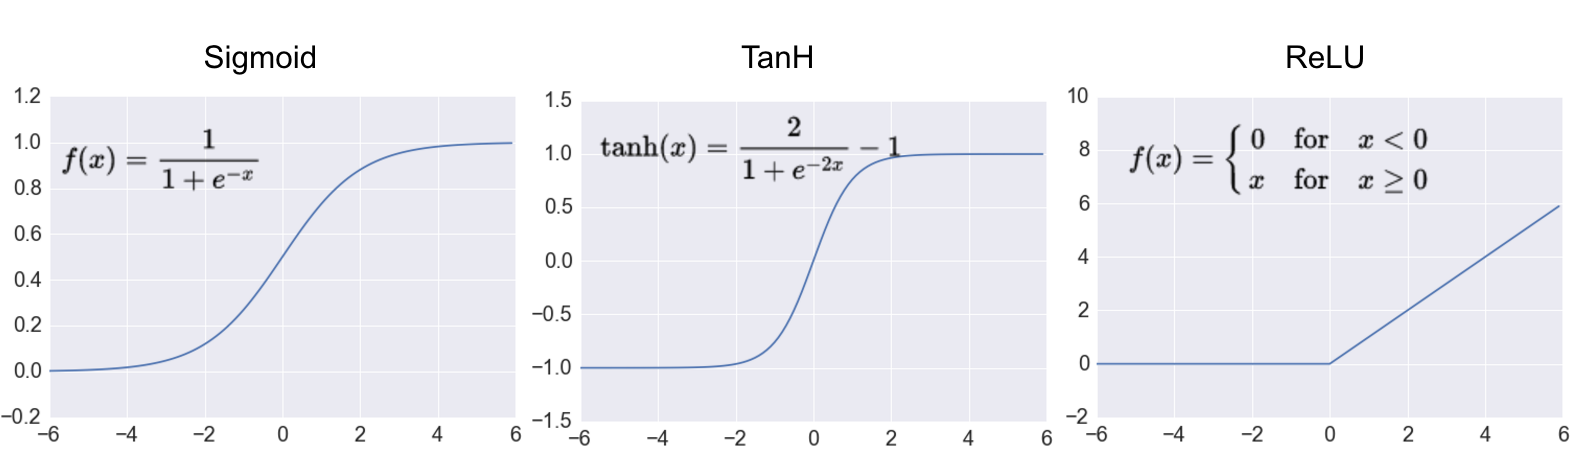
\includegraphics[width=0.8\textwidth]{images/marcoteorico/activfunct}
		\end{center}
		\begin{center}
		\caption{\small{Funciones de activación}}
		\vskip -0.2cm  
		{\small{Fuente: \cite{Adil}}}
		\end{center}
		\vspace{-1.5em}
		\end{figure}

		Actualmente, ReLU es la función de activación no lineal más utilizada \citep{cs231n}. La razón principal de esto es porque la red puede entrenar mucho más rápido (debido a la eficiencia computacional) sin hacer una diferencia significativa en la precisión. También ayuda a aliviar el problema del gradiente de fuga, que es el problema donde las capas inferiores de la red entrenan muy lentamente porque el gradiente de optimización	disminuye exponencialmente a través de las capas. La capa ReLU aplica la función ${f(x)} = {max (0, x)} $ a todos los valores en el volumen de entrada. En términos básicos, esta capa simplemente cambia todas las activaciones negativas a 0. Esta capa aumenta las propiedades no lineales del modelo y la red global sin afectar los campos receptivos de la capa convolucional. El hecho de que entradas en la función de activación de valores menores o iguales a cero resulten cero induce a la dispersión en las unidades ocultas, que según lo comentado anteriormente, produce representaciones dispersas las cuales se consideran más valiosas, \citep{RELU}. 
		
		\begin{figure}[H]
		\begin{center}
		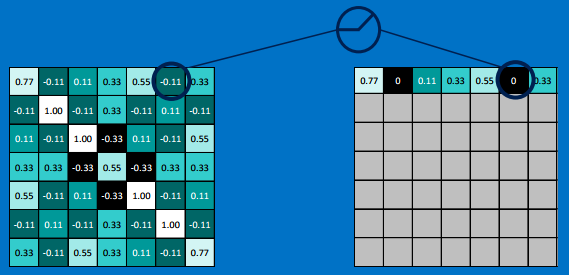
\includegraphics[width=0.8\textwidth, height=6cm]{images/marcoteorico/relu}
		\end{center}
		\begin{center}
		\caption{\small{Procedimiento de la función ReLU}}
		\vskip -0.2cm  
		{\small{Fuente: \cite{Rohrer}}}
		\end{center}
		\vspace{-1.5em}
		\end{figure}
		\vskip 0.4cm
		
		Es por ello que entre la capa de convolución y la capa de pooling puede encontrarse la capa ReLU, la cual está compuesta por neuronas que poseen una función de activación llamada Función Lineal Rectificada que deriva de la función de activación sigmoidal, pero tiene mayores ventajas que esta última y también de la tangencial. Las activaciones de ReLU se sobreponen más fácilmente que los sigmoides, esto los prepara muy bien para ser utilizados en combinación con la técnica DROPOUT.
		
		\vskip 0.4cm 
	\subsubsection {Técnica Dropout}
		
		Combinar las predicciones de muchos modelos diferentes es una forma muy exitosa de reducir los errores de prueba, pero parece ser demasiado costoso para las redes neuronales de gran tamaño debido a que pueden tardar varios días en entrenar. Sin embargo, dropout es una técnica de regularización que tiene por objetivo reducir el sobreajuste que puede darse durante el entrenamiento de una red neuronal. Esta técnica consiste en establecer a cero la salida de ciertas neuronas denominadas neuronas ocultas, las cuales son seleccionadas aleatoriamente en cada capa con una probabilidad comúnmente del 50\%. Las neuronas que se abandonan de esta manera no contribuyen al pase directo y no participan en las siguientes etapas de entrenamiento \citep{AulaDNN}.

		\begin{figure}[H]
		\begin{center}
		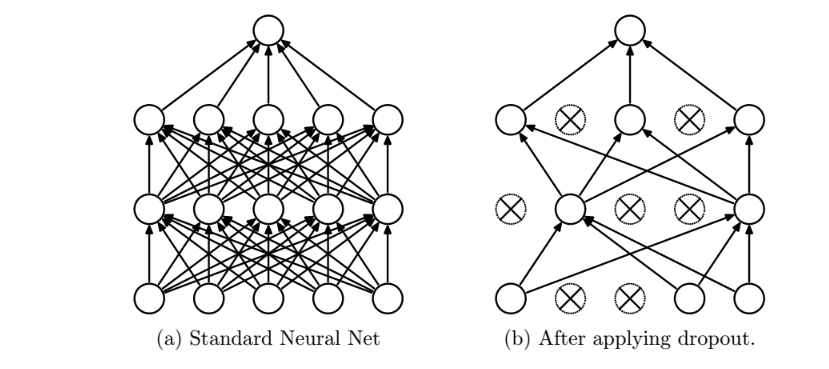
\includegraphics[width=0.7\textwidth]{images/marcoteorico/dropout_sample}
		\end{center}
		\begin{center}
		\caption{\small{En la izquierda la red neuronal común y a la derecha la red neuronal diluida producida por la aplicación de dropout}}
		{\small{Fuente: \cite{AulaDNN}}}
		\end{center}
		\vspace{-1.5em}
		\end{figure}
		

		\vskip 0.4cm 
		Por lo tanto, cada vez que se presenta una entrada, la red neuronal muestra una arquitectura diferente, pero todas estas arquitecturas comparten ponderaciones. Esta técnica reduce las co-adaptaciones complejas de las neuronas, ya que una neurona no puede depender de la presencia de otras neuronas particulares. Por lo tanto, se ve forzada a aprender características más robustas que son útiles en conjunción con muchos otros subconjuntos aleatorios provenientes de otras neuronas.
		\begin{figure}[H]
		\begin{center}
		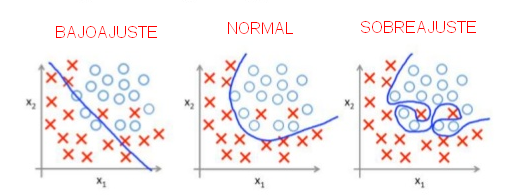
\includegraphics[width=0.8\textwidth]{images/marcoteorico/dropout}
		\end{center}
		\begin{center}
		\caption{\small{Procesos que pueden ocurrir durante entrenamiento. Dropout evita el sobreajuste}}
		\vskip -0.3cm  
		{\small{Fuente: Elaboración propia}}
		\end{center}
		\vspace{-1.5em}
		\end{figure}

		\vskip 0.4cm 
	\subsubsection {Capa de Agrupación(Pooling)}
		\vskip 0.4cm 

		Una variedad de cálculos que reducen la dimensión de un mapa de características se conocen como agrupación. La agrupación, que se aplica a cada canal por separado, permitiendo que la red sea robusta e invariante a pequeños cambios y distorsiones. La capa Pooling (también conocida como una capa de reducción de resolución) combina o agrupa un conjunto de valores en su campo receptivo generando un menor número de valores. Puede ser configurado en función del tamaño de su campo receptivo (por ejemplo, 2 x 2) y en función a la operación de agrupamiento (por ejemplo, máximo-max o promedio-average), como se muestra en Fig. 2.21. Normalmente, la agrupación se produce en bloques que no se solapan (es decir, el paso o stride es igual al tamaño de la agrupación) y usualmente se usa una stride mayor que uno cuando se quiere que haya una reducción en la dimensión de la representación (mapa de características).

		\begin{figure}[H]
		\begin{center}
		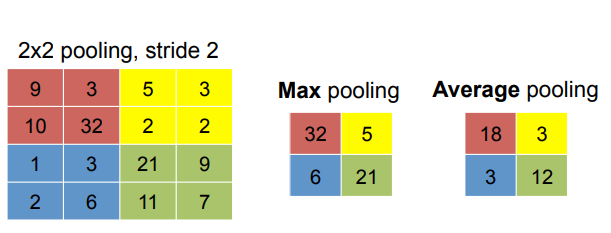
\includegraphics[width=0.8\textwidth]{images/marcoteorico/pooling}
		\end{center}
		\begin{center}
		\caption{\small{Formas de agrupamiento(pooling)}}
		\vskip -0.2cm  
		{\small{Fuente: \cite{caffe}}}
		\end{center}
		\vspace{-1.5em}
		\end{figure}

		Después de algunas capas ReLU, es común optar por aplicar una capa de agrupamiento. En esta categoría, la operación MAX (conocida como Max-pooling) es la más popular reduciendo progresivamente el tamaño espacial de la representación de una imagen (mapa de características) mientras conserva la información más importante en ella, esto se ejecuta con dos objetivos, el primero de reducir la cantidad de parámetros y reducir el cálculo en la red. Este último de gran importancia en el control del sobreajuste, \citep{Rohrer}.
		\vskip 0.4cm 
		La capa de agrupación opera independientemente en cada segmento de profundidad de la entrada y la cambia de tamaño espacialmente (reduce su resolución). El proceso matemático consiste en pasar una pequeña ventana(kernel) a través de una imagen y tomar el valor máximo de la ventana en cada paso. 


		\begin{figure}[H]
		\begin{center}
		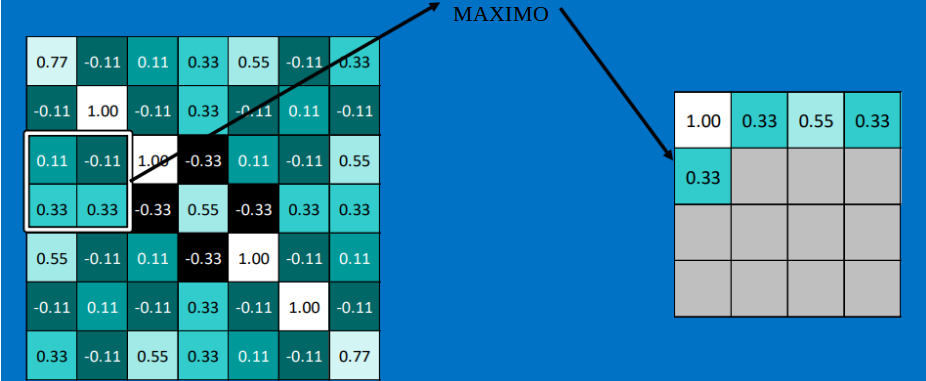
\includegraphics[width=0.75\textwidth]{images/marcoteorico/pool1}
		\end{center}
		\begin{center}
		\caption{\small{Operación MAX-pooling en capa de Agrupación}}
		\vskip -0.2cm  
		{\small{Fuente: \cite{Rohrer}}}
		\end{center}
		\vspace{-1.5em}
		\end{figure}

		Este proceso es aplicado para cada mapa de activación (salida de la capa de convolución). Análogamente con la capa de convolución, el resultado en esta capa es un conjunto de imágenes que muestran una versión agrupada de las imágenes de entrada.

		\begin{figure}[H]
		\begin{center}
		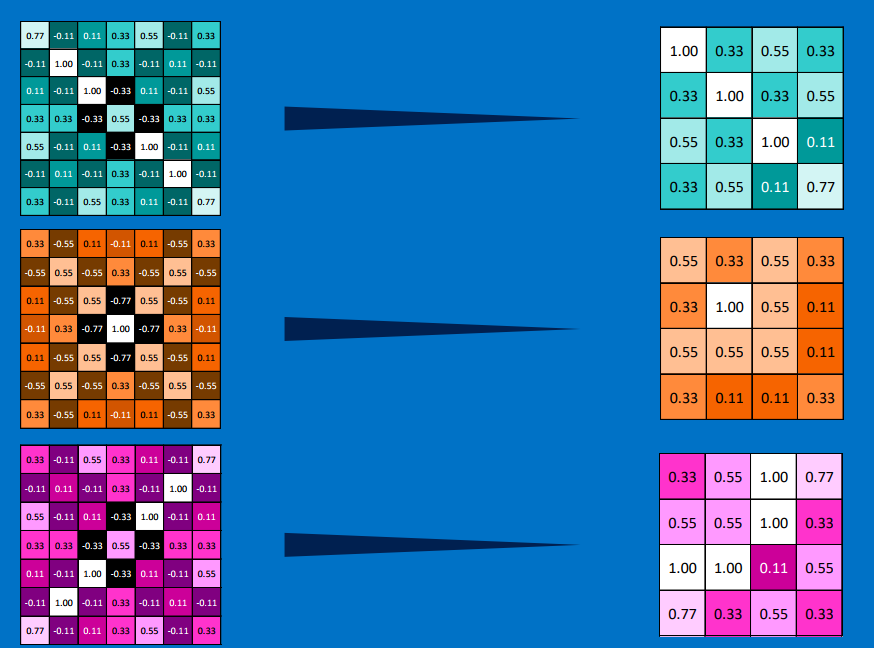
\includegraphics[width=0.6\textwidth]{images/marcoteorico/pool2}
		\end{center}
		\begin{center}
		\caption{\small{Resultado de Agrupación}}
		\vskip -0.2cm  
		{\small{Fuente: \cite{Rohrer}}}
		\end{center}
		\vspace{-1.5em}
		\end{figure}


		\noindent Esta capa pooling recibe como dato de entrada los parámetros:
		${W_{0}}\times{H_{0}}\times{D_{0}}$ \newline
		Produce un dato de salida con los siguientes parámetros: ${W_{1}}\times{H_{1}}\times{D_{1}}$\newline		
		% first column
		\begin{minipage}[t]{0.5\textwidth}
		En el que:
		\begin{center}
		 ${W_{1}} = \frac{{W_{0}} - F }{S} +1$ 
		\vskip 0.4cm 
		 ${H_{1}} = \frac{{H_{0}} - F }{S} +1$ 
		\vskip 0.4cm 
		 ${D_{1}} = {D_{0}}$ 
		 \end{center}
		\vskip 0.6cm 
		\end{minipage}
		%second column
		\begin{minipage}[t]{0.55\textwidth}
		Donde:
		\vskip 0.1cm 
		$W$ es el ancho (width) de la imagen, \vskip 0.4cm  
		$H$ es la altura (height) de la imagen,\vskip 0.4cm 
		$D$ es la profundidad (depth) de la imagen,\vskip 0.4cm 
		$F$ es la extensión espacial (spatial extent) del kernel,\vskip 0.4cm 
		$S$ es el paso (stride) del kernel,\vskip 0.4cm 
		\end{minipage}

		\begin{figure}[H]
		\begin{center}
		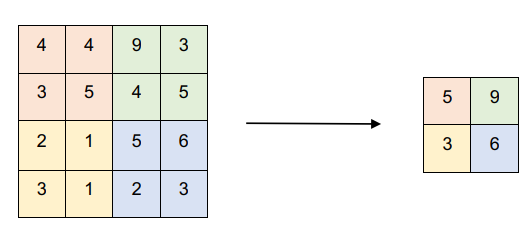
\includegraphics[width=0.45\textwidth]{images/marcoteorico/pool4}
		\end{center}
		\begin{center}
		\caption{\small{Max-pooling con filtro 2x2 y paso 2}}
		{\small{Fuente: Elaboración propia}}
		\end{center}
		\vspace{-1.5em}
		\end{figure}

	\subsection{Capa totalmente conectada (Fully-connected layer)}

		Luego de que los datos pasen por las capas de convolución, eventualmente, se tiene un mapa de características lo suficientemente pequeño y el contenido se aplasta en un vector de una sola dimensión. Hasta este punto, los datos ya son suficientes para un cierto grado de precisión en el reconocimiento de clases. Sin embargo, para obtener un mejor resultado en términos de complejidad y precisión, será usada al final de modelo, una capa neuronal totalmente conectada similar al Perceptrón Multicapa (MultilayerPerceptron - MLP), en el cual la neurona de salida se conecta a todas las neuronas de entrada y el peso de las conexiones son actualizadas usando el método de retropropagación, \citep{FCL}.

		El vector resultante obtenido de las capas de convolución será la entrada del MLP totalmente conectado con el cual se logrará obtener una salida determinada que represente la probabilidad de predicción del clasificador, esta será conseguida usando una función de activación diferente a la usada durante la convolución (función RELU), esta nueva función es conocida como función softmax, la cual es comúnmente usada en esta capa final del modelo \citep{Krizhevsky2012}.
	

En resumen, un modelo de red convolucional estará compuesto de varias capas y ejecutará las siguientes actividades:
\begin{figure}[H]
	\begin{center}
	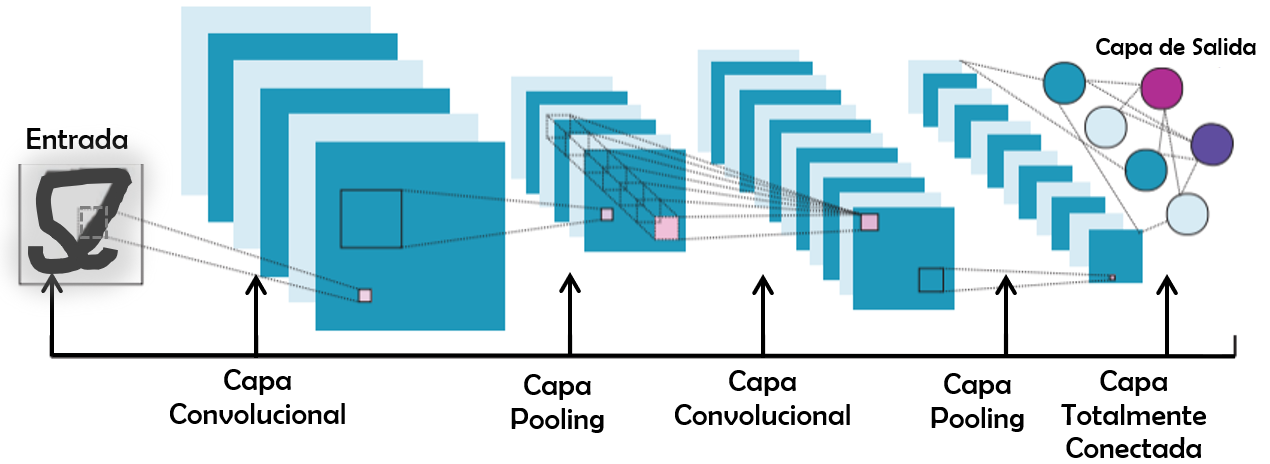
\includegraphics[width=0.8\textwidth]{images/marcoteorico/modelo}
	\end{center}
	\begin{center}
	\caption{\small{Modelo de red neuronal convolucional profunda}}
	{\small{Fuente: Elaboración propia}}
	\end{center}
	\vspace{-1.5em}
	\end{figure}

\begin{itemize}
	\item Se pasa una imagen de entrada a la primera capa convolucional, cuya salida se obtiene como un mapa de activación. Los filtros aplicados en la capa de convolución extraen características relevantes de la imagen de entrada para pasar más lejos.

	\item Los valores de cada filtro se irán ajustando durante el entrenamiento y en caso de que necesitemos retener el tamaño de la imagen, usamos el mismo relleno (padding cero), de lo contrario se usa el relleno válido ya que ayuda a reducir el número de características. \vspace{-0.5em}

	\item Las capas de agrupamiento se agregan para reducir aún más el número de parámetros.\vspace{-0.5em}

	\item Se agregan varias capas de convolución y agrupación antes de realizar la clasificación. \vspace{-0.5em}

	\item A medida que profundizamos en la red convolucional, se extraen características más específicas en comparación con una red lineal donde las características extraídas son más genéricas.

	\item La capa de salida en una CNN, como se mencionó anteriormente, es una capa totalmente conectada, donde la entrada de las otras capas se aplana y se envía para transformar la salida en el número de clases que desea la red. \vspace{-0.5em}

	\item La salida se genera a través de la capa de salida y se compara con una vector de resultados deseados para la generación de errores. Una función de pérdida se define en la capa de salida totalmente conectada para calcular el gradiente de error. \vspace{-0.5em}

	\item El error se retroproyecta para actualizar los valores de filtro (pesos) y sesgo (bias). \vspace{-0.5em}
	
	\item Finalmente, un ciclo de entrenamiento se completa en un solo pase hacia adelante y hacia atrás. Por lo que se tiene que repetir todo el proceso durante varias iteraciones para obtener mejores resultados.\vspace{-0.5em}

\end{itemize}

\newpage
\section{Entrenamiento y Validación}

	La red procesa los registros en los datos de entrenamiento uno a la vez, usando los pesos, biases y las funciones en las capas ocultas, luego compara las salidas resultantes con las salidas deseadas. Los errores se propagan a través del sistema, lo que hace que el sistema ajuste los pesos y biases que serán procesados en la siguiente iteración de entrenamiento. Este proceso ocurre una y otra vez para el mismo conjunto de datos, a medida que los pesos se ajustan (refinan) continuamente. Para realizar este proceso, existe un método de optimización muy popular denominado {\bf Descenso de gradiente} (Gradient Descent).

	\subsection{Descenso de Gradiente}

		Un gradiente mide cuánto cambia la salida de una función si se cambia un poco las entradas.

		En el caso del entrenamiento de una red neuronal, el gradiente simplemente mide el cambio en todos los pesos con respecto al cambio en el error. El gradiente se puede representar como la pendiente de una función, cuanto más alto es el gradiente, más pronunciada es la pendiente y más rápido puede aprender un modelo. Pero si la pendiente es cero, el modelo deja de aprender. Dicho matemáticamente, un gradiente es una derivada parcial con respecto a sus entradas, \citep{gradient}.

		El descenso de gradiente es un algoritmo de optimización iterativa utilizado al entrenar un modelo de aprendizaje automático, basado en una función convexa, que ajusta sus parámetros iterativamente para minimizar la función de pérdida (error) hasta su mínimo local, \citep{gradient}.

		La idea detrás del descenso de gradiente es disminuir de forma gradual, pero constante, el error de salida ajustando los pesos y biases. Intuitivamente, se conoce que si un cambio en un peso aumentará o disminuirá el error, entonces queremos disminuir o aumentar ese peso. Matemáticamente, representa el cambio en el error dado un cambio de unidad en el peso:

		\begingroup\makeatletter\def\f@size{20.8}\check@mathfonts
		\begin{center}
		$ \frac{{\partial E}}{\partial w_{ij}}$
		\end{center}
		\begin{center}
		{\small{Ecuación de la derivada del error con respecto al peso}}
		\end{center}
		\endgroup
		
		Una vez que encontremos esta derivada, actualizamos el peso a través de la siguiente fórmula:

		\begingroup\makeatletter\def\f@size{17.8}\check@mathfonts
		\begin{center}
		$  \triangle w_{ij} = -\eta\frac{{\partial E}}{\partial w_{ij}} $
		\end{center}
		\begin{center}
		{\small{Representación del ajuste del peso, donde $\eta$ es la tasa de aprendizaje}}
		\end{center}
		\endgroup

		La tasa de Aprendizaje suele disminuir gradualmente durante las épocas de la fase de entrenamiento. Si actualizamos todos los pesos usando esta misma fórmula, esto equivale a moverse en la dirección de descenso más pronunciado a lo largo de la superficie de error, de ahí el nombre, descenso de gradiente.
		\begin{figure}[H]
		\begin{center}
		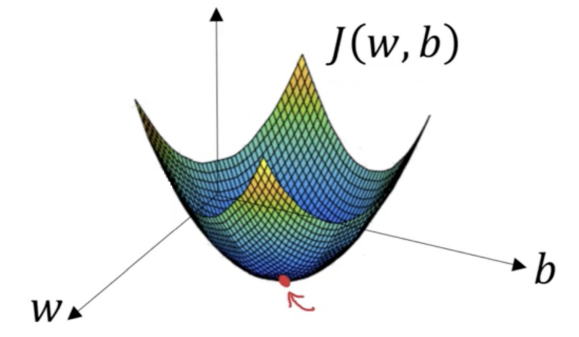
\includegraphics[width=0.45\textwidth]{images/desarrollo/entrenamiento/gradient}
		\end{center}
		\begin{center}
		\caption{\small{Descenso de Gradiente a través de ajustes en los pesos y biases}}
		\vspace{-0.5em}
		{\small{Fuente: \cite{gradientimg}}}
		\end{center}
		\vspace{-1.5em}
		\end{figure}

		Se tienen diversos tipos de descenso de gradiente, estos son:
		%con el objetivo principal de optimizar la funcion de error o pérdida de la red y por consecuente garantizar que el modelo neuronal pueda generalizar las clasificaciones a realizar. 
		\subsubsection{Gradiente Descendiente por Lotes (Batch Gradient Descent - BGD)}
		
			Calcula el error para cada ejemplo dentro del conjunto de datos de entrenamiento, pero el modelo se actualiza solo después de que se hayan evaluado todos los ejemplos de entrenamiento. Todo este proceso es como un ciclo y se denomina época de entrenamiento.

		\subsubsection{Gradiente Descendiente Estocástico (Stochastic Gradient Descent - SGD)}

			Por el contrario, hace esto para cada ejemplo de entrenamiento dentro del conjunto de datos. Esto significa que actualiza los parámetros para cada ejemplo de entrenamiento, uno por uno. Esto puede hacer que el SGD sea más rápido que el Descenso de gradiente por lotes, dependiendo del problema. Una ventaja es que las actualizaciones frecuentes nos permiten tener una tasa de mejora bastante detallada. El hecho es que las actualizaciones frecuentes son más costosas desde el punto de vista computacional que el enfoque del BGD y la frecuencia de esas actualizaciones también puede generar gradientes ruidosos, lo que puede hacer que la tasa de error salte, en lugar de disminuir lentamente.

			%El MOMENTUM es otro argumento en el optimizador SGD que podríamos ajustar para obtener una convergencia más rápida. Ayuda al vector de parámetros a aumentar la velocidad en cualquier dirección con un descenso constante del gradiente para evitar oscilaciones. Una elección típica de momento es entre 0.5 a 0.9.

		\subsubsection{Mini-batch Gradient Descent}

			Es el método de gradiente más usado, ya que es una combinación de los conceptos de SGD y BGD, y es el usado en esta investigación. Simplemente divide el conjunto de datos de entrenamiento en pequeños lotes y realiza una actualización para cada uno de estos lotes. Por lo tanto, es más rápido que los métodos anteriormente mencionados y agrega ruido al proceso de aprendizaje, ayudando a mejorar el error de generalización. Además, al evaluar pequeños lotes, se seleccionan aleatoriamente diversos ejemplos evitando procesar ejemplos muy similares que no contribuyen mucho al aprendizaje. %crea un equilibrio entre la robustez del descenso del gradiente estocástico y la eficiencia del descenso del gradiente discontinuo.

			\begin{figure}[H]
			\begin{center}
			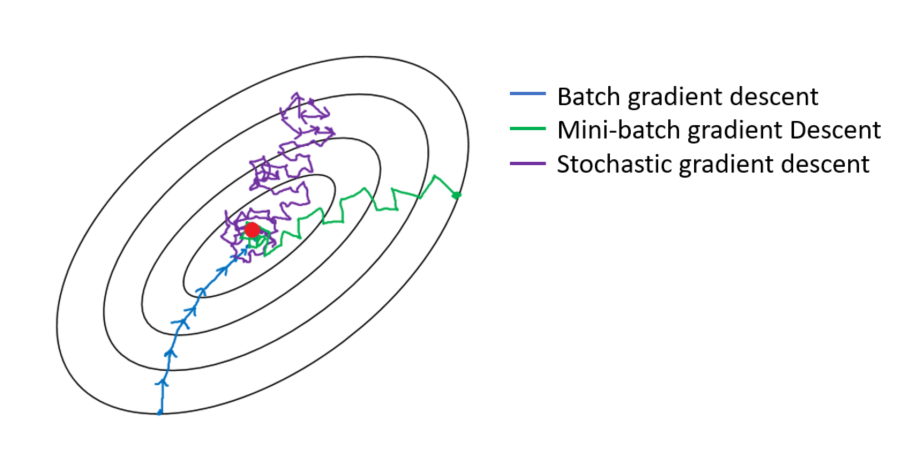
\includegraphics[width=0.65\textwidth]{images/desarrollo/gradientDescent}
			\end{center}
			\begin{center}
			\caption{\small{Variantes del descenso del gradiente y su dirección hacia el mínimo error}}
			\vspace{-0.5em}
			{\small{Fuente: \cite{Imad}}}
			\end{center}
			\vspace{-1.5em}
			\end{figure}


	\subsection{Tasa de Aprendizaje (Learning Rate)}
		Uno de los hiperparámetros clave durante el entrenamiento de una red neuronal es la velocidad/tasa de aprendizaje para el descenso del gradiente.
		Este parámetro puede entenderse como el tamaño del paso en la optimización para minimizar la función de pérdida de la red, es decir, es un parámetro que determina cuánto influye un paso de actualización en el valor actual de los pesos, \citep {AdamImg}. %Es decir, determina el tamaño del paso en el que el gradiente cae en la dirección máxima de la pendiente.

		\begin{figure}[H]
		%\begin{center}
		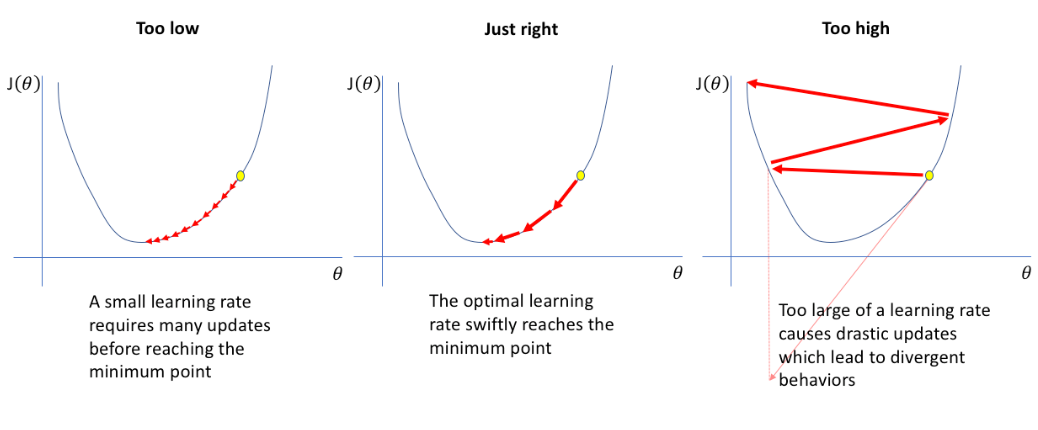
\includegraphics[width=1\textwidth]{images/desarrollo/entrenamiento/LR}
		%\end{center}
		\begin{center}
		\caption{\small{Establecimiento de la Tasa de Aprendizaje}}
		\vspace{-0.5em}
		{\small{Fuente: \cite{AdamImg}}}
		\end{center}
		\vspace{-1.5em}
		\end{figure}

		Cuando la tasa de aprendizaje es demasiado pequeña, es necesario realizar muchas iteraciones de aprendizaje; pero cuando la tasa de aprendizaje es demasiado grande, el resultado se moverá hacia adelante y hacia atrás en ambos sentidos de los valores extremos(oscila), y no se podrá lograr la solución óptima como puede ser observado en la figura 2.28.

		Debido a esto es que al entrenar redes neuronales profundas, a menudo es útil reducir la tasa de aprendizaje a medida que avanza el entrenamiento y no mantenerlo constante y así evitar la divergencia (punto a partir del cual la pérdida ya no se reduce y en lugar de eso comienza a incrementarse), \cite{AdamImg}.


		\begin{figure}[H]
		%\begin{center}
		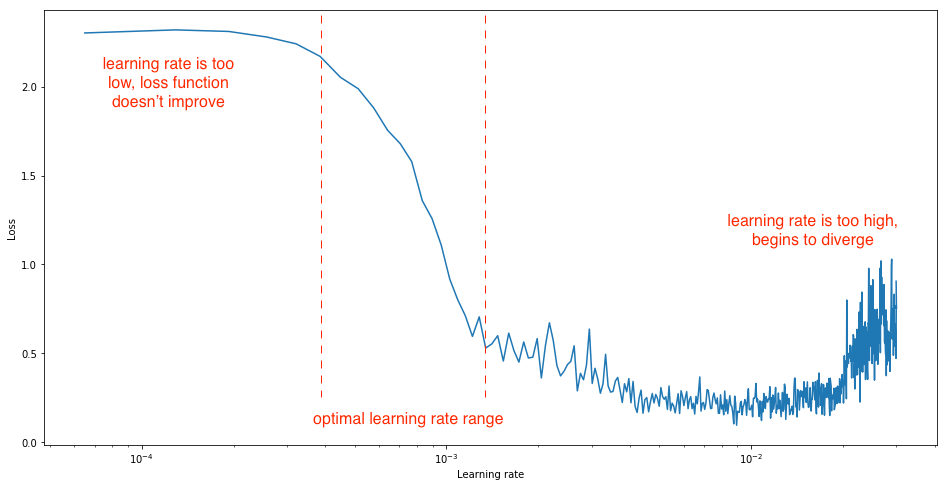
\includegraphics[width=1\textwidth]{images/desarrollo/entrenamiento/lr_finder}
		%\end{center}
		\begin{center}
		\caption{\small{Comportamientos en la reducción de la Tasa de Aprendizaje}}
		{\small{Fuente: \cite{AdamImg}}}
		\end{center}
		\vspace{-1.5em}
		\end{figure}

		Reduciendo lentamente la tasa de aprendizaje a lo largo del tiempo ayuda a acelerar el aprendizaje. Esto es lo que se conoce como tasa de decaimiento de aprendizaje {\bf(learning rate decay)}.
			\begin{figure}[H]
				\begin{center}
				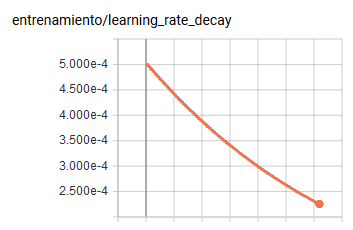
\includegraphics[width=0.6\textwidth,height=5.5cm]{images/desarrollo/entrenamiento/LR_decay} 
				\end{center}
				\begin{center}
				\caption{\small{Ejemplo de Tasa de decaimiento de aprendizaje por época  }}
				\vspace{-0.5em}
				{\small{\fontsize{10}{16.8}\selectfont {Fuente: Elaboración propia}}}
				\end{center}
				\vspace{-1.5em}
			\end{figure}
		Sin embargo, el optimizador Gradient Descent (en cualquiera de sus tipos) con una tasa de decaimiento de aprendizaje, no es usado a menudo para entrenar redes neuronales profundas ya que genera un desafío el determinar los hiperparámetros que deben definirse de antemano y dependen en gran medida del tipo de modelo y problema. Además de que la misma tasa de aprendizaje se aplica a todas las actualizaciones de los parámetros. Por lo que opta en usar optimizadores más avanzados que tienen una tasa de convergencia más rápida, adaptable a diversas situaciones y son conocidos como optimizadores de descenso de gradiente de segundo orden; tales como optimizador Adagrad, Adadelta, RMSprop, Adam, entre otros. 

		%AdaGrad or adaptive gradient allows the learning rate to adapt based on parameters. It performs larger updates for infrequent parameters and smaller updates for frequent one. Because of this it is well suited for sparse data (NLP or image recognition). Another advantage is that it basically illiminates the need to tune the learning rate. Each parameter has its own learning rate and due to the peculiarities of the algorithm the learning rate is monotonically decreasing. This causes the biggest problem: at some point of time the learning rate is so small that the system stops learning.AdaDelta resolves the problem of monotonically decreasing learning rate in AdaGrad. In AdaGrad the learning rate was calculated approximately as one divided by the sum of square roots. At each stage you add another square root to the sum, which causes denominator to constantly decrease. In AdaDelta instead of summing all past square roots it uses sliding window which allows the sum to decrease. RMSprop is very similar to AdaDelta. Adam or adaptive momentum is an algorithm similar to AdaDelta. But in addition to storing learning rates for each of the parameters it also stores momentum changes for each of them separately

		En esta investigación se usa el método Adam como optimizador de segundo orden.

	\subsection{Optimizador ADAM}
	
		Es un algoritmo de optimización de tasa de aprendizaje adaptativo que ha sido diseñado específicamente para el entrenamiento de redes neuronales profundas; el nombre Adam deriva de Estimación del Momento Adaptativo \citep {Adam},

		Permite que la tasa de aprendizaje se adapte según los parámetros y realiza actualizaciones más grandes para parámetros infrecuentes y actualizaciones más pequeñas para los frecuentes. Debido a esto, es adecuado para datos dispersos, como lo es en el procesamiento de lenguaje natural o en el reconocimiento de imágenes. Otra ventaja es que básicamente simplifica la necesidad de ajustar la tasa de aprendizaje debido a que cada parámetro tiene su propia tasa de aprendizaje. 
		\begin{figure}[H]
				\begin{center}
				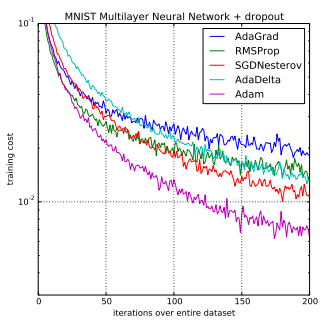
\includegraphics[width=0.6\textwidth, height=0.4\textheight]{images/desarrollo/adam} 
				\end{center}
				\begin{center}
				\caption{\small{Comparación de Adam con otros algoritmos de optimización que entrenan a un perceptrón multicapa}}
				\vspace{-0.5em}
				{\small{{Fuente: \cite{Adam}}}}
				\end{center}
				\vspace{-1.5em}
			\end{figure}

	\subsection{Validación Cruzada}
	
		%Cross-entropy loss, or log loss, measures the performance of a classification model whose output is a probability value between 0 and 1. Cross-entropy loss increases as the predicted probability diverges from the actual label. So predicting a probability of .012 when the actual observation label is 1 would be bad and result in a high loss value. A perfect model would have a log loss of 0.

		Para el entrenamiento, el conjunto de datos se divide en un subconjunto de entrenamiento y otro para validación. La división en subgrupos de entrenamiento y validación generalmente se realiza de manera aleatoria, para garantizar que ambos subconjuntos sean muestras aleatorias de la misma distribución. Puede ser razonable realizar un muestreo estratificado, lo que significa asegurar que cada clase esté presente en la misma proporción en los subconjuntos de entrenamiento y prueba. En esta investigación se trabajará con 2 tipos de muestreos (balanceado/estratificado y no balanceado).

		El subconjunto de validación es utilizado para evaluar el desempeño del entrenamiento en diferentes arquitecturas del modelo (diferentes topologías), para luego escoger una de ellas. Este conjunto de validación se usa para verificar si el error está dentro de algún rango y no se usa directamente para ajustar los pesos, por el contrario, \textbf{se usa para indicar el número óptimo de neuronas ocultas o determina el punto de parada para el entrenamiento}.  Por lo tanto, el modelo es entrenado sobre el conjunto de entrenamiento completo y la capacidad de generalización es medida en el conjunto de validación. 

		La validación cruzada o cross-validation es una técnica utilizada para evaluar los resultados de un análisis estadístico y garantizar que son independientes de la partición entre datos de entrenamiento y validación, \citep{moore2001cross}. En problemas de clasificación, debido a que los datos se dividen en clases finitas, es natural pensar que la categoría al cual pertenece cierto resultado se dará a través de probabilidades. En probabilidad, la entropía cruzada es la distancia entre las dos distribuciones de probabilidad y se usa generalmente como la función de pérdida. Es por ello que el resultado de la validación cruzada representa la pérdida de la entropía del conjunto de datos. La entropía se suele utilizar en la teoría de la información para medir la pureza o impureza de un conjunto determinado. La pregunta a la que responde es: ¿Cuánto diferente esos elementos son entre sí? 

			\begingroup\makeatletter\def\f@size{17.8}\check@mathfonts
			\begin{center}
			$H(p,q) = -\sum_{\forall x} p(x) log(q(x))$
			\end{center}
			\begin{center}
			{\small{Fórmula de entropía cruzada con dos distribuciones sobre la variable discreta $x$, donde $q(x)$ es la estimación para la clasificación verdadera $p(x)$}}
			\end{center}
			\endgroup		

		Para una red neuronal, normalmente verá la ecuación escrita en una forma donde $y$ es el vector de datos reales y la variable $\hat{y}$ (o algún otro valor tomado directamente de la última salida de la capa) es la estimación, y se vería así para un solo ejemplo:
			
			\begingroup\makeatletter\def\f@size{17.8}\check@mathfonts
			\begin{center}
			$L = - \mathbf{y} \cdot log(\mathbf{\hat{y}})$
			\end{center}
			%\begin{center}
			%{\small{El valor es independiente de cómo la probabilidad restante se divide entre clases incorrectas}}
			%\end{center}
			\endgroup		
		
		A menudo esta ecuación es promediada sobre todos los ejemplos como una función de costo. No siempre se cumple estrictamente en las descripciones, pero generalmente una función de pérdida es de nivel inferior y describe cómo una sola instancia o componente determina un valor de error, mientras que una función de costo es de nivel superior y describe cómo se evalúa un sistema completo para la optimización. Una función de costo basada en pérdida de clasificación de múltiples clases para un conjunto de datos de tamaño N podría verse así:
		
			\begingroup\makeatletter\def\f@size{17.8}\check@mathfonts
			\begin{center}
			$J = - \frac{1}{N}(\sum_{i=1}^{N} \mathbf{y_i} \cdot log(\mathbf{\hat{y}_i}))$
			\end{center}
			\begin{center}
			{\small{Cálculo de la función de costo en la validación de clasificación de datos}}
			\end{center}
			\endgroup		
	

		Es por ello que la función de costo dada por la validación cruzada ayuda para decidir cuándo se debe terminar el entrenamiento de una red, \citep{AulaMLP}. Usualmente se utiliza el error cuadrático medio como función de pérdida para medir el rendimiento de un modelo de regresión. Sin embargo, en casos de clasificación, el cálculo de la entropía cruzada es preferible, ya que produce un aprendizaje más rápido al no causar saturación de las neuronas de salida (proceso cuando la entrada es próxima a cero, generando que el peso correspondiente se ajusta lentamente),  \citep{AulaDNN}. La pérdida de entropía cruzada aumentará a medida que la probabilidad prevista diverge de la clasificación real. Por lo tanto, un modelo casi perfecto tendría una pérdida de entropía cercana a cero, \citep{crossMSE}.
		


	\subsection{Función Softmax}
		Conocida también como función exponencial normalizada, es la función de activación utilizada en la última capa de una red neuronal. La salida de una red neuronal completamente conectada no es una distribución de probabilidad, sin embargo, el uso de esta función ayuda a obtenerla. Por lo que esta función permitirá estimar la probabilidad de que la imagen de entrada pertenezca a cada una de las clases al realizar una normalización con el objetivo que el valor de cada neurona esté limitado entre cero y uno y así permitir que los resultados de las neuronas de salida sumen a uno, \citep{Bishop}. 

			\begingroup\makeatletter\def\f@size{17.8}\check@mathfonts
			\begin{center}
			${\displaystyle P(y=j\mid \mathbf {x} )={\frac {e^{\mathbf {x} ^{\mathsf {T}}\mathbf {w} _{j}}}{\sum _{k=1}^{K}e^{\mathbf {x} ^{\mathsf {T}}\mathbf {w} _{k}}}}}$
			\end{center}
			\begin{center}
			{\small{Función Softmax}}
			\end{center}
			\endgroup
			
		Esto se puede ver como la composición de K funciones lineales ${x} \mapsto \mathbf {x} ^{\mathsf {T}}\mathbf {w} _{1},\ldots ,\mathbf {x} \mapsto \mathbf {x} ^{\mathsf {T}}\mathbf {w} _{K}$, donde ${\mathbf {x} ^{\mathsf {T}}\mathbf {w}}$ denota el producto interno de $x$(entrada) y $w$(peso).	La operación es equivalente a aplicar un operador lineal definido por $ w $ a vectores $ x $, transformando así la entrada original, probablemente altamente dimensional (reales arbitrarios), en vectores K-dimensional de valores reales en el rango [0, 1] que suman 1. \citep{Bishop}. 

		Esta función permite que al estar normalizadas las salidas de la segunda capa totalmente conectada, pueda ser aplicada la validación cruzada y conocer la pérdida de entropía.

	
	\subsection{Método de Regularización L2}
		La regularización es una técnica que realiza ligeras modificaciones en el algoritmo de aprendizaje, de manera que el modelo se generaliza mejor. En la regularización, lo que se hace normalmente es mantener el mismo número de funciones, pero se reduce la magnitud de los coeficientes(pesos de neuronas), sin embargo, el método de Regularización L2 o también conocido como Regresión Lasso, trata de agregar un término adicional(lambda) a la función de coste, la cual penaliza parametrizaciones con pesos más elevados, es decir, reduce el coeficiente(peso) de las funciones menos importantes a cero eliminando así algunas características. Por lo tanto, mantiene los pesos pequeños, evitando que la red utilice pesos que no necesite realmente, logrando que la red no se ajuste demasiado al conjunto de entrenamiento \citep{AulaMLP}.

		Si $L(\theta, D)$ es la función de coste, $\theta$ es el conjunto de parámetros libres y $D$ es un ejemplo de entrenamiento, entonces a la función de pérdida regularizada será:

			\begingroup\makeatletter\def\f@size{15.8}\check@mathfonts
			\begin{center}
			$E(\theta,D) =L(\theta,D) +\lambda R(\theta)$
			\end{center}
			\endgroup
		

		Donde $R(\theta)$ caracteriza la complejidad del modelo y $\lambda$ representa la proporción de la coste total del modelo, generalmente $\lambda$ es una constante y estará cerca de 0 porque si $\lambda$ es demasiado grande, conducirá a un ajuste insuficiente (underfitting). Por otro lado, para evitar el exceso de ajuste (overfitting) cuando se tiene una gran cantidad de características en su conjunto de datos, no optimizamos directamente $L(\theta,D)$ (la entropía cruzada), sino que optimizamos $L(\theta,D) +\lambda R(\theta)$.

		En esta investigación se usará una constante {\bf lambda($\lambda$) = 0.0001}. La regularización L2 incluye los pesos de las capas totalmente conectadas, y normalmente no incluye a los biases (sesgos). La intuición detrás de esto es que el bias contribuye al overfitting (sobreajuste) y no estaría agregando ningún nuevo grado de libertad al modelo, \citep{AulaMLP}.



%============================================================================================================%============================================================================================================%============================================================================================================%============================================================================================================


\section{Método de la investigación}

\subsection{ Tipo de investigación}
	De acuerdo al fin que se persigue es una investigación de tipo tecnológica y de acuerdo al diseño es una investigación experimental de tipo cuantitativa donde se analizará el rendimiento del modelo algorítmico.

\subsection{Variables de la Investigación}
		
		\subsubsection{Variable Dependiente}
		\indent Reconocimiento automático de señales de tránsito vehicular
		\subsubsection {Variable Independiente}
		\indent Modelo basado en el aprendizaje profundo de redes neuronales convolucionales	
		
\subsection{Indicadores}
		\renewcommand{\baselinestretch}{2}
		Los indicadores nos permiten realizar mediciones y a su vez determinan la validez de la hipótesis planteada en la presente investigación. El desempeño de la clasificación se puede verificar con los siguientes seis indicadores: 
		\begin{table}[H]
		\centering
		\caption{\small{Indicadores para la investigación}}
		\begin{tabular}{|>{\small}c|>{\small}c|>{\small}c|}
		\hline
		{\ul \textbf{Indicador}} & {\ul \textbf{Descripción}} & {\ul \textbf{Instrumento}} \\ \hline
		\multirow{2}{*}{\begin{tabular}[c]{@{}c@{}}Tasa de Verdaderos Positivos\\ (Efectividad - Sensibilidad)\end{tabular}} & \multirow{2}{*}{$ \frac{Verdaderos\,Positivos}{{Verdaderos\,Positivos}+{Falsos\,Negativos}}$} & \multirow{2}{*}{\begin{tabular}[c]{@{}c@{}}Matriz de\\ Confusión\end{tabular}} \\
		 &  &  \\ \hline
		\multirow{2}{*}{\begin{tabular}[c]{@{}c@{}}Tasa de Verdaderos Negativos \\ (Especificidad)\end{tabular}} & \multirow{2}{*}{$ \frac{Verdaderos\,Negativos}{{Verdaderos\,Negativos}+{Falsos\,Positivos}}$} & \multirow{2}{*}{\begin{tabular}[c]{@{}c@{}}Matriz de\\ Confusión\end{tabular}} \\
		 &  &  \\ \hline
		 \multirow{2}{*}{\begin{tabular}[c]{@{}c@{}}Valor Predictivo Positivo \\ (Precisión)\end{tabular}} & \multirow{2}{*}{$ \frac{Verdaderos\,Positivos}{{Verdaderos\,Positivos}+{Falsos\,Positivos}}$} & \multirow{2}{*}{\begin{tabular}[c]{@{}c@{}}Matriz de\\ Confusión\end{tabular}} \\
		 &  &  \\ \hline
		\multirow{2}{*}{\begin{tabular}[c]{@{}c@{}}Tasa de Acierto \\ (Exactitud)\end{tabular}} & \multirow{2}{*}{$ \frac{Verdaderos\,Positivos+Verdaderos\,Negativos}{Total\,de\,Imagenes}$} & \multirow{2}{*}{\begin{tabular}[c]{@{}c@{}}Matriz de\\ Confusión\end{tabular}} \\
		 &  &  \\ \hline
		 \multirow{2}{*}{\begin{tabular}[c]{@{}c@{}}Curvas PR \\ (Precision - Recall)\end{tabular}} & \multirow{2}{*}{Relación entre Efectividad(Recall) y Precision} & \multirow{2}{*}{\begin{tabular}[c]{@{}c@{}}Matriz de\\ Confusión\end{tabular}} \\
		 &  &  \\ \hline
		%\multirow{2}{*}{\begin{tabular}[c]{@{}c@{}}Tiempo de\\ Procesamiento\end{tabular}} & \multirow{2}{*}{$S= \frac{\sum_{i=1}^{Total} tiempo_{i}}{Total\,de\,muestras}$} & \multirow{2}{*}{\begin{tabular}[c]{@{}c@{}}Cronometro\\ Computacional\end{tabular}} \\
		\multirow{2}{*}{\begin{tabular}[c]{@{}c@{}}Curvas ROC \\ (Receiver Operating Characteristic)\end{tabular}} & \multirow{2}{*}{Relación entre Efectividad y Especificidad} & \multirow{2}{*}{\begin{tabular}[c]{@{}c@{}}Matriz de\\ Confusión\end{tabular}} \\
		&  &  \\ \hline 		 
		\end{tabular}
		\begin{center}
				\vskip 0.3cm
				{\small{Fuente: Elaboración propia.}}
				\end{center}
		\vspace{-1.0em}
		\end{table}

	\newpage
\subsection{Recolección de Datos para la Construcción del Modelo}
		%\renewcommand{\baselinestretch}{1.2}
		\subsubsection{Técnica de Recolección}
		\begin{enumerate}		
			\item[]   {Revisión de la literatura (análisis de documentos)}.
		\end{enumerate}

		\subsubsection{Población}
		\begin{enumerate}		
			\item[] Existen diversas arquitecturas de redes neuronales convolucionales usadas para propósitos específicos. La idea principal es que al principio la arquitectura de la red neuronal toma como entrada una imagen y su especificación de dimensiones en 3 valores (largo, ancho y profundidad). Capas convolucionales y capas de activación(optimización) se apilan juntas y luego son seguidas por capas de agrupamientos. Esta estructura se usa comúnmente y se repite hasta que la entrada (imagen) se fusiona espacialmente a un tamaño pequeño. Después de eso, se envía a capas completamente conectadas y la salida de la última capa completamente conectada, que está al final de la arquitectura, produce los puntajes de clase de la imagen de entrada.
		\end{enumerate}
		
	
		\subsubsection{Muestra}
		\begin{enumerate}		
		\item[] Para el proceso de diseño e implementación de arquitecturas a elaborar se tomarán en cuenta dos modelos mundialmente conocidos e importantes:
		\end{enumerate}
				
		\begin{enumerate}
		\item[] {\bf \underline {Arquitectura AlexNet }}\newline
			AlexNet fue desarrollado por \cite{Krizhevsky2012}. Esta arquitectura hizo que las redes convolucionales fueran populares cuando en el 2012, AlexNet en el concurso ImageNet LSVRC-2012 superó significativamente a todas las otras redes neuronales a través de su diseño de red convolucional profunda para clasificar 1.2 millones de imágenes en 1000 clases diferentes. Ganó el desafío al obtener un error de 15.3\% y el segundo lugar (que no fue una variación de una CNN) obtuvo una tasa de error alrededor del 26,2\%.

			Compuesta aproximadamente de 60 millones de neuronas, la entrada consiste en una imagen de 224x224 pixeles en formato RGB (3 canales). La arquitectura consta de 8 capas, las primeras cinco capas son convolucionales y el resto son capas totalmente conectadas. La salida de cada capa convolucional y cada capa completamente conectada se activa a través de la función no linear RELU.  Presenta filtros de tamaño 11x11, 5x5 , 3x3 y capas de agrupación(pooling), siendo lo más destacable el uso de dropout como técnica de regularización y el uso del proceso de Data Augmentation para conseguir esos excelentes resultados.
		\end{enumerate}

		\begin{enumerate}
		\item[] {\bf \underline {Arquitectura Inception}}\newline
			Es una arquitectura de red neuronal convolucional profunda, creada por un grupo de investigación de Google que fue responsable de establecer el nuevo estado del arte de la técnica para la clasificación y detección en la competencia de reconocimiento visual a gran escala ImageNet 2014(ILSVRC14). 
			\vskip 0.1cm
			El principal sello distintivo de esta arquitectura es la utilización mejorada de los recursos informáticos dentro de la red. Esto fue logrado gracias al aumento de la profundidad y el ancho de la red mientras se mantiene el costo computacional constante, reduciendo el número de parametros usados en AlexNet(60 millones) a 4 millones. Para optimizar la calidad, las decisiones para elaborar la arquitectura se basaron en el principio Hebbiano y la intuición de funciones de procesamiento a escala múltiple, \citep{Inception}.  Lo que significa que la salida de las capas convolucionales no solo se envía a la capa posterior, sino que también se ramifica y se introduce al clasificador (capa totalmente conectada). Una encarnación particular utilizada en la competencia ILSVRC14 es llamada GoogLeNet, una red de 22 capas de profundidad, cuya calidad se evalúa en el contexto de reconocimiento y detección, logrando una tasa de error del 6.67\%, muy cercano al rendimiento a nivel humano.
		\end{enumerate}
		%====================================================================================
		% subsection Recolección de Datos para la Construcción del Modelo (end)

	\subsection{Recolección de Datos para el Entrenamiento y Evaluación del Modelo}
		
		\subsubsection{Técnica de Recolección}
		\begin{enumerate}		
			\item[]  Revisión de la literatura (análisis de documentos) y captura de imágenes del Perú a través de la aplicación Google Maps.
		\end{enumerate}
		\newpage
		\subsubsection{Población} 
		\begin{enumerate}
		\item[]				
		{\bf *) Área:} Imágenes de Señales de Seguridad Vial.\vskip 0.1cm
		{\bf *) Categoría:} Tránsito Vehicular Vertical.\vskip 0.1cm
		{\bf *) Subcategoría:} Señales reguladoras, preventivas e informativas.\vskip 0.1cm
		\end{enumerate}

		\begin{enumerate}		
			\item[]  La población es infinita para esta investigación, debido al número infinito de formas distintas en que una señal de tránsito puede ser capturada. Se tomarán en cuenta imágenes donde se muestren señales de tránsito vehicular del tipo vertical en sus 3 subcategorías.
		\end{enumerate}

		\subsubsection{Muestra} 
		\begin{enumerate}		
			\item[]	Existe una colección(dataset) que se ajusta a las características de nuestra población y será usada para conseguir el objetivo de la investigación, principalmente porque cuenta con abundantes imágenes lo que conforma una muestra representativa y necesaria para hacer generalizaciones. 
		\end{enumerate}

		\begin{enumerate}
			\item[]  {\bf \underline {Señales de Tránsito de Alemania}}\newline
			Conjunto de datos creados a partir de aproximadamente 10 horas de video grabados durante el día mientras se conducía en diferentes tipos de carreteras en Alemania. De las secuencias del video fueron extraídas imágenes de señales de tránsito en formato RGB cuyas dimensiones varían entre 15x15 y 250x250 pixeles. En esta colección se obtuvieron un total de 39209 imágenes distribuidas en 43 clases.  \citep{Stallkamp-IJCNN-2011} 
		\end{enumerate}

		%\item[B)] {\bf Señales de Tránsito de Bélgica} \citep{Timofte-MVA-2011} \newline
		%	Conjunto de datos creados con a la captura simultánea de imágenes durante el día realizada por 8 cámaras mientras se conducía aproximadamente a 35Km/h, con el objetivo de obtener una localización 3D y un refinamiento simultáneo. Las señales de tránsito fueron capturados a una distancia de menos de 50 metros y almacenadas en formato PPM cuyas dimensiones varían entre 25x30 y 260x250 pixeles. En esta colección se obtuvieron un total de 7125 imágenes distribuidas en 62 clases.
		
		
		\begin{enumerate}
			\item[]  {\bf \underline {Señales de Tránsito de Perú}}\newline
			Conjunto de aproximadamente 614 imágenes originalmente tomadas de la aplicación Google Maps agrupadas en 7 categorías. Dado que la población de imágenes es infinita, se optó por usar un muestreo aleatorio simple para poblaciones desconocidas con un nivel de confianza del 95\% y un error de muestreo del 4\%.
		
			\vskip 0.4cm
			\begingroup\makeatletter\def\f@size{17.8}\check@mathfonts
			\begin{center}
				${\bf n} ={\bf \frac{z^2pq}{e^2}}$
			\end{center}
			\endgroup
		
			En el que:\vskip 0.1cm
			\begin{itemize}
				\item $n$ = tamaño de muestra
				\item $z$ = Coeficiente de confiabilidad 95\% al que corresponde (1.96)
				\item $pq$ = Varianza de la población, ponemos la varianza mayor posible porque a mayor varianza hará falta una muestra mayor (0.25)
				\item $e$ = Error muestral (0.04)
			\end{itemize}
		\end{enumerate}
		%====================================================================================
		% subsection Recolección de Datos para el Entrenamiento y Evaluación del Modelo (end)
\newpage
\subsection{Etapas de la investigación} 
	El desarrollo de la investigación comprenderá las siguientes etapas de trabajo a saber:

		\begin{enumerate}

		\item[a)]	Investigación bibliográfica de los diferentes temas necesarios para la elaboración de la investigación, tales como dispositivos de control de tránsito, vehículos autónomos, sistemas avanzados de asistencia al conductor, aprendizaje profundo (deep learning), procesamiento de imágenes, entre otros.
		
		\item[b)]	Búsqueda de los principales casos de éxito en el reconocimiento de señales de tránsito a través de trabajos de investigación en el Perú como también en otros países.

		\item[c)]	Recolección de imágenes de señales de tránsito vehicular que se utilizarán en el desarrollo de la investigación.

		\item[d)]	Análisis e implementación de diversas técnicas de procesamiento de imágenes que serán aplicadas al dataset recolectado con la finalidad de contribuir en el diseño inicial del modelo convolucional.

		\item[e)]	Puesto a que las redes neuronales son heurísticas por naturaleza (requieren un constante ajuste de hiperparámetros para obtener un óptimo resultado), se realizarán diferentes diseños de arquitecturas de modelos convolucionales y se escogerá el modelo que otorgue los mejores resultados.
		
		\item[f)]	Para el análisis de resultados, se pretende usar una Matriz de confusión. A través de esta matriz, se pueden conocer los indicadores conocidos con tasa de sensibilidad, especificidad, precisión y valores estadísticos del espacio ROC (Receiver Operating Characteristic), métricas usadas comúnmente para evaluar la calidad del modelo reconocedor.
		
		\end{enumerate}

		\subsubsection{Metodología para el diseño del Modelo}

			Se utilizará la metodología propuesta por Tammy Noergard (T. Noergaard, 2005) , la cual toma mucha de las claves de las metodologías conocidas como Rational Unified Process (RUP), Attribute Driven Desing (ADD), Object Oriented Process (OOP) y el Model Driven Architecture (MDA), pero las simplifica. La siguiente figura muestra las diferentes fases de la metodología.
			
			\begin{figure}[H]
			\begin{center}
			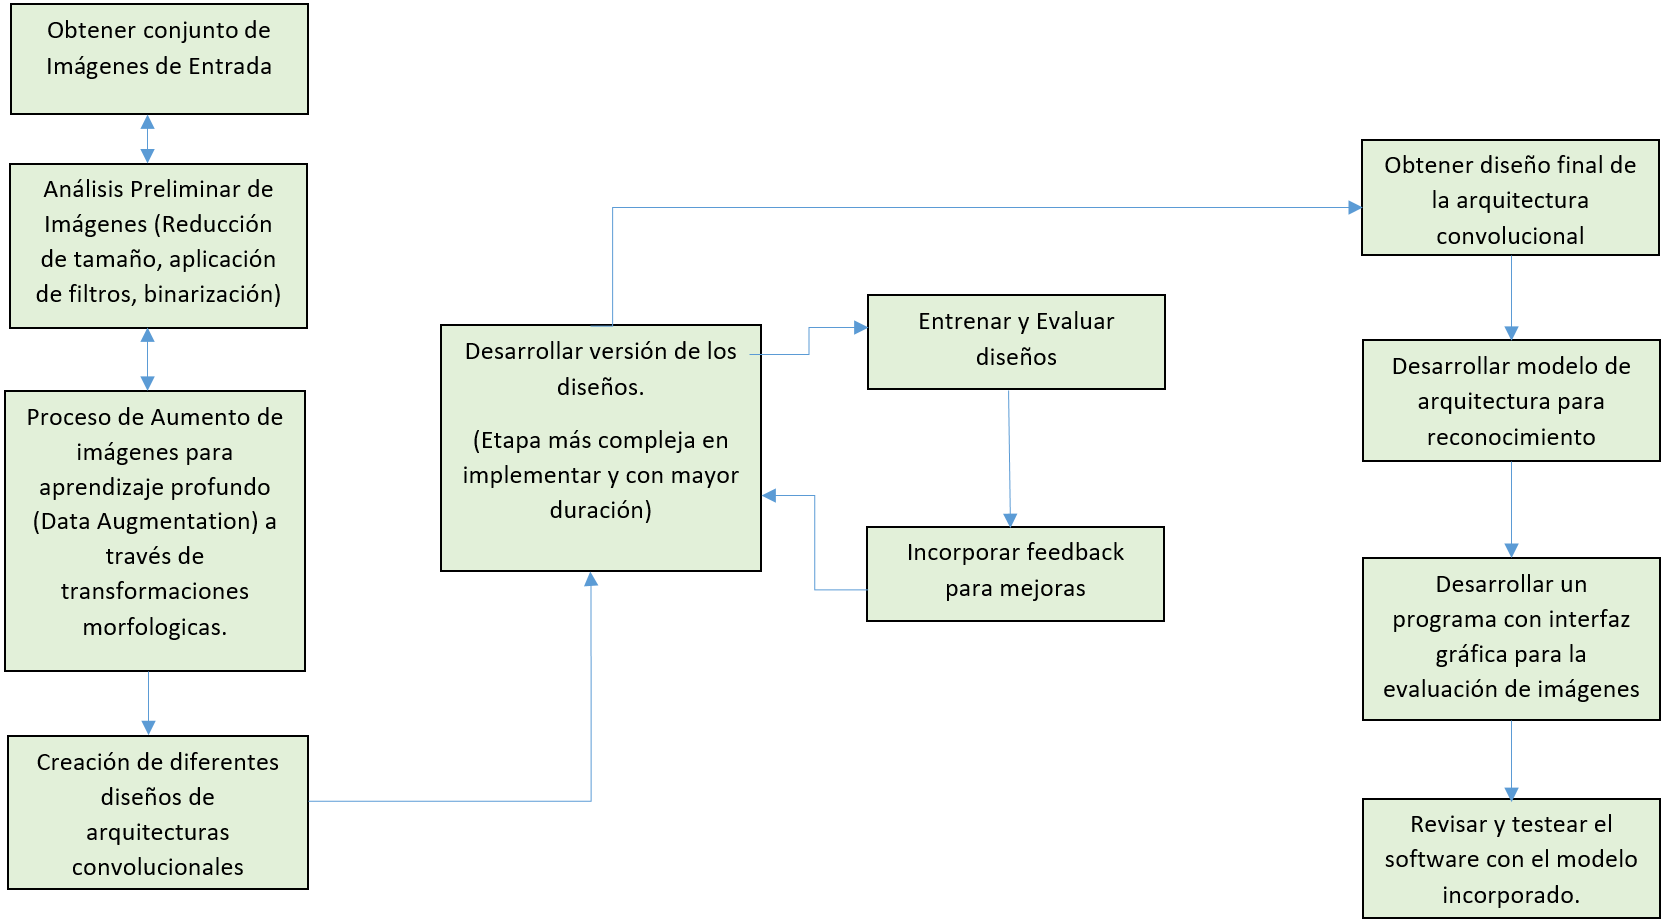
\includegraphics[width=0.9\textwidth, height=0.4\textheight]{images/intro/disenho}
			\end{center}
			\begin{center}
			\vskip 0.6cm	
			\caption{\small{Diseño del Modelo del Ciclo de Vida del Desarrollo}}
			\vspace{-1.5em}
			{\small{Fuente: Elaboración propia}}
			\end{center}
			
			\end{figure}


% subsection Etapas de la investigación (end)



	